\begin{enumerate}[label=\thesection.\arabic*,ref=\thesection.\theenumi]
\item Find the number of terms in each of the following APs. 
\begin{enumerate}
    \item 7, 13, 19, ... 205

    \item 18, 15$\frac{1}{2}$, 13, ... -47
\end{enumerate}
\solution
\iffalse
\let\negmedspace\undefined
\let\negthickspace\undefined
\documentclass[journal,12pt,twocolumn]{IEEEtran}
\usepackage{cite}
\usepackage{amsmath,amssymb,amsfonts,amsthm}
\usepackage{algorithmic}
\usepackage{graphicx}
\usepackage{textcomp}
\usepackage{xcolor}
\usepackage{txfonts}
\usepackage{listings}
\usepackage{enumitem}
\usepackage{mathtools}
\usepackage{gensymb}
\usepackage{comment}
\usepackage[breaklinks=true]{hyperref}
\usepackage{tkz-euclide} 
\usepackage{listings}
\usepackage{gvv}                                        
\def\inputGnumericTable{}                                 
\usepackage[latin1]{inputenc}                                
\usepackage{color}                                            
\usepackage{array}                                            
\usepackage{longtable}                                       
\usepackage{calc}                                             
\usepackage{multirow}                                         
\usepackage{hhline}                                           
\usepackage{ifthen}                                           
\usepackage{lscape}
\usepackage{placeins}
\usepackage{xparse}


\newtheorem{theorem}{Theorem}[section]
\newtheorem{problem}{Problem}
\newtheorem{proposition}{Proposition}[section]
\newtheorem{lemma}{Lemma}[section]
\newtheorem{corollary}[theorem]{Corollary}
\newtheorem{example}{Example}[section]
\newtheorem{definition}[problem]{Definition}
\newcommand{\BEQA}{\begin{eqnarray}}
\newcommand{\EEQA}{\end{eqnarray}}
\newcommand{\define}{\stackrel{\triangle}{=}}
\theoremstyle{remark}
\newtheorem{rem}{Remark}



\begin{document}

\bibliographystyle{IEEEtran}
\vspace{3cm}

\Large\title{NCERT Question 10.5.2.5}
\large\author{EE23BTECH11032 - Kaustubh Parag Khachane $^{*}$% <-this % stops a space
}
\maketitle
\newpage
\bigskip

\renewcommand{\thefigure}{\theenumi}
\renewcommand{\thetable}{\theenumi}
\large\textbf{Question 10.5.2.5} : \normalsize Find the number of terms in each of the following APs. Then express each term as x\brak{n} and find the z transform, ROC and plot the graph for x\brak{n}: 
\begin{enumerate}
    \item 7, 13, 19, ... 205

    \item 18, 15$\frac{1}{2}$, 13, ... -47
\end{enumerate}


\solution
\fi
\begin{table}[ht] 
\centering
\setlength{\extrarowheight}{8pt}
\begin{tabular}{|c|l|l|} 
 \hline
  \textbf{Parameter} & \textbf{Used to denote } & \textbf{Values} \\ 
 \hline
 $x_{i}$\brak{n} & $n^{th}$ term of $i^{th}$ series $\brak{i =\brak{1,2}}$  & $\brak{x_{i}\brak{0} + nd_{i}}u\brak{n}$ \\
 \hline
$x_{i}$\brak{0} & First term of $i^{th} $ AP &\multicolumn{1}{|p{1.5cm}|}{\centering $x_{1}\brak{0} = 7$ \\ $x_{2}\brak{0} = 18$ }\\
 \hline
  $d_{i}$ & Commmon difference of $i^{th}$ AP&\multicolumn{1}{|p{1.5cm}|}{\centering $d_{1} = 6 $ \\ $d_{2} = -2.5$}\\
 \hline

\end{tabular}
 \vspace{4mm}
 \caption{Parameter Table}
 \label{tab:table0}
\end{table}

The number of terms in the AP x\brak{n} is given by: 
\begin{align}  \label{eq:eq12}
    \frac{x\brak{n} - x\brak{0}}{d} + 1
\end{align}
\begin{align}
    &X_i(z) = \frac{x_i\brak{0}}{1 - z^{-1}} + d_i\frac{z^{-1}}{\brak{1-z^{-1}}^2} \text{ , for i=1,2} \label{eq:eq3}\\
    &\text{ROC : $\abs{z} > 1$ as it is an AP}   
\end{align}
\begin{enumerate}
    \item 
\begin{align}
x_{1}\brak{n} &= \brak{7 + \brak{n}6}u\brak{n}
\end{align}
Using the values in \tabref{tab:table0} and equation \eqref{eq:eq12},
\begin{align}
    k_1 = \frac{205 - 7}{6} + 1 = 34
\end{align}

Using the values in \tabref{tab:table0} and equation \eqref{eq:eq3} :
\begin{align}
 X_1\brak{z} = \frac{7 - z^{-1}}{\brak{1-z^{-1}}^2}
\end{align}

ROC is $\abs{z} > 1$
 
   \item
   
\begin{align}
    x_{2}\brak{n} &= \brak{18 + n\brak{-2.5}u\brak{n}}
\end{align}

Using the values in \tabref{tab:table0} and equation \eqref{eq:eq12},
\begin{align}
    k_2 = \frac{-47 - 18}{-2.5} + 1 = 27
\end{align}

Using the values in \tabref{tab:table0} and equation \eqref{eq:eq3} :
\begin{align} 
 X_2\brak{z} = \frac{18 - \brak{20.5}z^{-1}}{\brak{1 - z^{-1}}^2}
\end{align}

ROC is $\abs{z} > 1$.

\begin{figure}[!ht]
\centering
\begin{center}
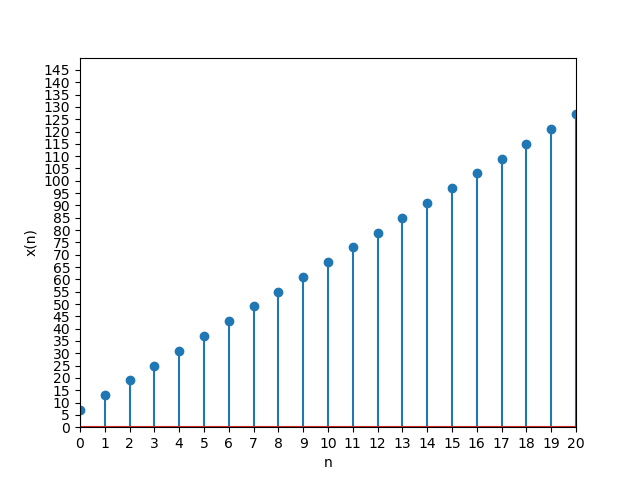
\includegraphics[width=\columnwidth]{ncert-maths/10/5/2/5/figs/Figure_1}
\caption{Plot of $x_1\brak{n}$}
\end{center}
\end{figure}

\begin{figure}[!ht]
\centering
\begin{center}
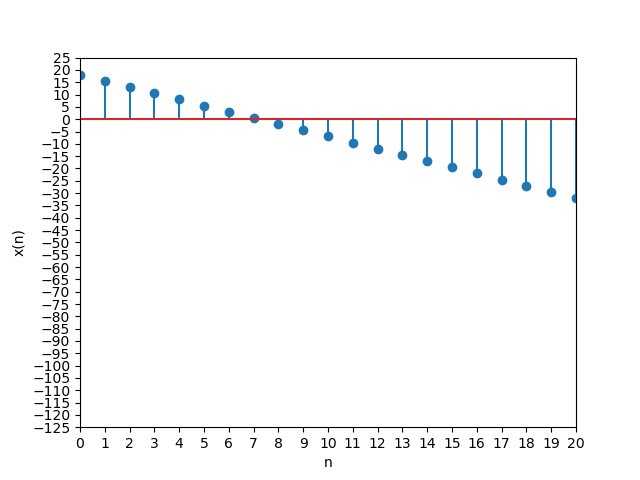
\includegraphics[width=\columnwidth]{ncert-maths/10/5/2/5/figs/Figure_2}
\caption{Plot of $x_2\brak{n}$}
\end{center}
\end{figure}

\end{enumerate}
%\end{document}



\item For what value of $ n$, are the $ nth$ terms of two A.Ps: 63, 65, 67,\dots and 3, 10, 17,\dots equal?
\solution
\iffalse
\let\negmedspace\undefined
\let\negthickspace\undefined
\documentclass[journal,12pt,twocolumn]{IEEEtran}
\usepackage{cite}
\usepackage{amsmath,amssymb,amsfonts,amsthm}
\usepackage{algorithmic}
\usepackage{graphicx}
\usepackage{textcomp}
\usepackage{xcolor}
\usepackage{txfonts}
\usepackage{listings}
\usepackage{enumitem}
\usepackage{mathtools}
\usepackage{gensymb}
\usepackage{comment}
\usepackage[breaklinks=true]{hyperref}
\usepackage{tkz-euclide}
\usepackage{listings}
\usepackage{gvv}
\def\inputGnumericTable{}
\usepackage[latin1]{inputenc}
\usepackage{color}
\usepackage{array}
\usepackage{longtable}
\usepackage{calc}
\usepackage{multirow}
\usepackage{hhline}
\usepackage{ifthen}
\usepackage{lscape}

\newtheorem{theorem}{Theorem}[section]
\newtheorem{problem}{Problem}
\newtheorem{proposition}{Proposition}[section]
\newtheorem{lemma}{Lemma}[section]
\newtheorem{corollary}[theorem]{Corollary}
\newtheorem{example}{Example}[section]
\newtheorem{definition}[problem]{Definition}
\newcommand{\BEQA}{\begin{eqnarray}}
\newcommand{\EEQA}{\end{eqnarray}}
\newcommand{\define}{\stackrel{\triangle}{=}}
\theoremstyle{remark}
\newtheorem{rem}{Remark}
\begin{document}

\bibliographystyle{IEEEtran}
\vspace{3cm}

\title{NCERT Discrete 10.5.2 -15}
\author{EE23BTECH11057 - Shakunaveti Sai Sri Ram Varun$^{}$% &lt;-this % stops a space
}
\maketitle
\newpage
\bigskip

\vspace{2cm}
\textbf{Question: }
For what value of $ n$, are the $ nth$ terms of two A.Ps: 63, 65, 67,\dots and 3, 10, 17,\dots equal?\\
\vspace{0.5cm}
\textbf{Solution}:
\fi

\begin{table}[htbp] 
\centering
\begin{tabular}{|c|c|c|c|}
    \hline
    \textbf{Parameter} & \textbf{Sub-question} & \textbf{Description} & \textbf{Value} \\
    \hline
    \multirow{2}{*}{$x_i\brak{0}$} & $x_1\brak{0}$ & $1^{st}$ term of $1^{st}$ A.P. & 63 \\
    \cline{2-4}
    & $x_2\brak{0}$ & $1^{st}$ term of $2^{nd}$ A.P. & \phantom{0}3 \\
    \hline
    \multirow{2}{*}{$d_i$} & $d_1$ & Common difference of $1^{st}$ A.P. & \phantom{0}2 \\
    \cline{2-4}
    & $d_2$ & Common difference of $2^{nd}$ A.P. & \phantom{0}7 \\
    \hline
\end{tabular}

\caption{input values}
\label{tab: table10.5.2.15}
\end{table}
\begin{align}
x_i\brak{n} &= x\brak{0}u\brak{n} + dnu\brak{n}\\
X\brak{z} &= \frac{x\brak{0}}{1-z^{-1}} + \frac{dz^{-1}}{\brak{1-z^{-1}}^{2}} \quad |z|>1
\end{align}
\begin{enumerate}
\item
\begin{align}
x_1\brak{n} &= 63u\brak{n} + 2nu\brak{n} \\
%To find $ X_1\brak{z}$:
X_1\brak{z} &= \frac{63}{1-z^{-1}} + \frac{2z^{-1}}{\brak{1-z^{-1}}^{2}}  \quad |z|>1
\end{align}
\item
\begin{align}
x_2\brak{n} &= 3u\brak{n} + 7nu\brak{n}\\ 
%To find $ X_2\brak{z}$ :\\
X_2\brak{z} &= \frac{3}{1-z^{-1}} + \frac{7z^{-1}}{\brak{1-z^{-1}}^{2}} \quad |z|>1
\end{align}
\item

given,
\begin{align}
 x_1\brak{n} &= x_2\brak{n}\\
\therefore 63 + 2n &= 7n+3\\
\implies n &=12
\end{align}
\begin{figure}[h!]
    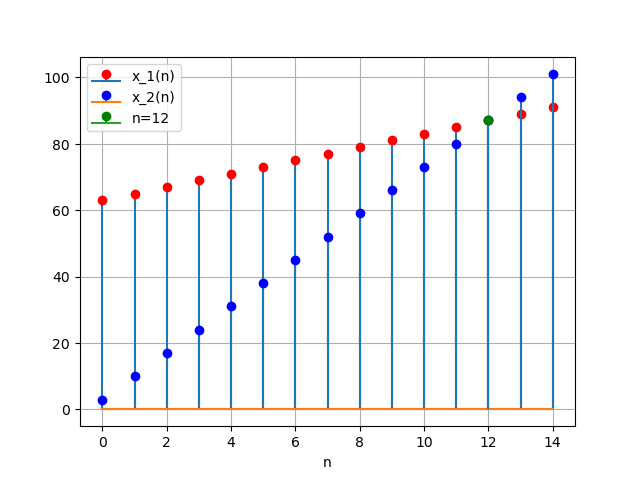
\includegraphics[width = \columnwidth]{ncert-maths/10/5/2/15/figs/Figure_1.png}
    \caption{Graphs of $ x_1\brak{n}$ and $ x_2\brak{n}$ and both are equal at $ n=12$}
    \label{fig: fig10.5.2.15}
\end{figure}
\end{enumerate}



\item Two APs have the same common difference.The difference between their $100${th} terms is 100,what is the difference between their $1000${th} terms?

\solution
\let\negmedspace\undefined
\let\negthickspace\undefined
\documentclass[journal,12pt,onecolumn]{IEEEtran}
\usepackage{cite}
\usepackage{amsmath,amssymb,amsfonts,amsthm}
\usepackage{algorithmic}
\usepackage{graphicx}
\usepackage{textcomp}
\usepackage{xcolor}
\usepackage{txfonts}
\usepackage{listings}
\usepackage{enumitem}
\usepackage{mathtools}
\usepackage{gensymb}
\usepackage[breaklinks=true]{hyperref}
\usepackage{tkz-euclide} % loads  TikZ and tkz-base
\usepackage{listings}



\newtheorem{theorem}{Theorem}[section]
\newtheorem{problem}{Problem}
\newtheorem{proposition}{Proposition}[section]
\newtheorem{lemma}{Lemma}[section]
\newtheorem{corollary}[theorem]{Corollary}
\newtheorem{example}{Example}[section]
\newtheorem{definition}[problem]{Definition}
%\newtheorem{thm}{Theorem}[section] 
%\newtheorem{defn}[thm]{Definition}
%\newtheorem{algorithm}{Algorithm}[section]
%\newtheorem{cor}{Corollary}
\newcommand{\BEQA}{\begin{eqnarray}}
\newcommand{\EEQA}{\end{eqnarray}}
\newcommand{\define}{\stackrel{\triangle}{=}}
\theoremstyle{remark}
\newtheorem{rem}{Remark}
%\bibliographystyle{ieeetr}
\begin{document}
%
\providecommand{\pr}[1]{\ensuremath{\Pr\left(#1\right)}}
\providecommand{\prt}[2]{\ensuremath{p_{#1}^{\left(#2\right)} }}        % own macro for this question
\providecommand{\qfunc}[1]{\ensuremath{Q\left(#1\right)}}
\providecommand{\sbrak}[1]{\ensuremath{{}\left[#1\right]}}
\providecommand{\lsbrak}[1]{\ensuremath{{}\left[#1\right.}}
\providecommand{\rsbrak}[1]{\ensuremath{{}\left.#1\right]}}
\providecommand{\brak}[1]{\ensuremath{\left(#1\right)}}
\providecommand{\lbrak}[1]{\ensuremath{\left(#1\right.}}
\providecommand{\rbrak}[1]{\ensuremath{\left.#1\right)}}
\providecommand{\cbrak}[1]{\ensuremath{\left\{#1\right\}}}
\providecommand{\lcbrak}[1]{\ensuremath{\left\{#1\right.}}
\providecommand{\rcbrak}[1]{\ensuremath{\left.#1\right\}}}
\newcommand{\sgn}{\mathop{\mathrm{sgn}}}
\providecommand{\abs}[1]{\left\vert#1\right\vert}
\providecommand{\res}[1]{\Res\displaylimits_{#1}} 
\providecommand{\norm}[1]{\left\lVert#1\right\rVert}
%\providecommand{\norm}[1]{\lVert#1\rVert}
\providecommand{\mtx}[1]{\mathbf{#1}}
\providecommand{\mean}[1]{E\left[ #1 \right]}
\providecommand{\cond}[2]{#1\middle|#2}
\providecommand{\fourier}{\overset{\mathcal{F}}{ \rightleftharpoons}}
\newenvironment{amatrix}[1]{%
  \left(\begin{array}{@{}*{#1}{c}|c@{}}
}{%
  \end{array}\right)
}
%\providecommand{\hilbert}{\overset{\mathcal{H}}{ \rightleftharpoons}}
%\providecommand{\system}{\overset{\mathcal{H}}{ \longleftrightarrow}}
	%\newcommand{\solution}[2]{\textbf{Solution:}{#1}}
\newcommand{\solution}{\noindent \textbf{Solution: }}
\newcommand{\cosec}{\,\text{cosec}\,}
\providecommand{\dec}[2]{\ensuremath{\overset{#1}{\underset{#2}{\gtrless}}}}
\newcommand{\myvec}[1]{\ensuremath{\begin{pmatrix}#1\end{pmatrix}}}
\newcommand{\mydet}[1]{\ensuremath{\begin{vmatrix}#1\end{vmatrix}}}
\newcommand{\myaugvec}[2]{\ensuremath{\begin{amatrix}{#1}#2\end{amatrix}}}
\providecommand{\rank}{\text{rank}}
\providecommand{\pr}[1]{\ensuremath{\Pr\left(#1\right)}}
\providecommand{\qfunc}[1]{\ensuremath{Q\left(#1\right)}}
	\newcommand*{\permcomb}[4][0mu]{{{}^{#3}\mkern#1#2_{#4}}}
\newcommand*{\perm}[1][-3mu]{\permcomb[#1]{P}}
\newcommand*{\comb}[1][-1mu]{\permcomb[#1]{C}}
\providecommand{\qfunc}[1]{\ensuremath{Q\left(#1\right)}}
\providecommand{\gauss}[2]{\mathcal{N}\ensuremath{\left(#1,#2\right)}}
\providecommand{\diff}[2]{\ensuremath{\frac{d{#1}}{d{#2}}}}
\providecommand{\myceil}[1]{\left \lceil #1 \right \rceil }
\newcommand\figref{Fig.~\ref}
\newcommand\tabref{Table~\ref}
\newcommand{\sinc}{\,\text{sinc}\,}
\newcommand{\rect}{\,\text{rect}\,}
%%
%	%\newcommand{\solution}[2]{\textbf{Solution:}{#1}}
%\newcommand{\solution}{\noindent \textbf{Solution: }}
%\newcommand{\cosec}{\,\text{cosec}\,}
%\numberwithin{equation}{section}
%\numberwithin{equation}{subsection}
%\numberwithin{problem}{section}
%\numberwithin{definition}{section}
%\makeatletter
%\@addtoreset{figure}{problem}
%\makeatother

%\let\StandardTheFigure\thefigure
\let\vec\mathbf


\bibliographystyle{IEEEtran}
\title{SEQUENCES}
\author{EE23BTECH11011- Batchu Ishitha$^{*}$% <-this % stops a space
}
\maketitle




\bigskip

\renewcommand{\thefigure}{\theenumi}
\renewcommand{\thetable}{\theenumi}
%\renewcommand{\theequation}{\theenumi}

Q:Two APs have the same common difference.The difference between their $100${th} terms is 100,what is the difference between their $1000${th} terms?

\solution

\begin{align}
x(n) &= \{x(0)+nd\}u(n) \\
 x(99) - y(99) &= 100 \\
\implies (x(0) + 99d) - (y(0) + 99d) &= 100
 \\
\implies x(0) - y(0) &= 100
\end{align}

\begin{align}
x(n) - y(n) &= (x(0) + nd) - (y(0) + nd)\\
&= x(0) - y(0) \\
&= 100 \\
\implies x(999)-y(999)&=100 
\end{align}

\begin{table}[!ht]
    \centering
        \begin{table}[ht]
    \centering
    \begin{tabular}{|c|c|c|}
        \hline
        Parameter & Value & Description \\
        \hline
        $x(0)$ & 5 & First term of AP \\
        $d$ & 1.75 & Common difference of AP \\
        $x(n)$ & 20.75 & $n^{th}$ term of AP \\
        \hline
    \end{tabular}
    \vspace{2mm}
    \caption{Parameter List}
    \label{tab:simple.10.5.2.20}
\end{table}

    \caption{input parameters}
    \label{tab:10_5_3_12}
\end{table}
Let 
\begin{align}
x(n)&= \lbrace 101,106,111,...\rbrace \\
y(n)&= \lbrace 1,6,11,... \rbrace
\end{align}


\begin{figure}[h]
    \centering
    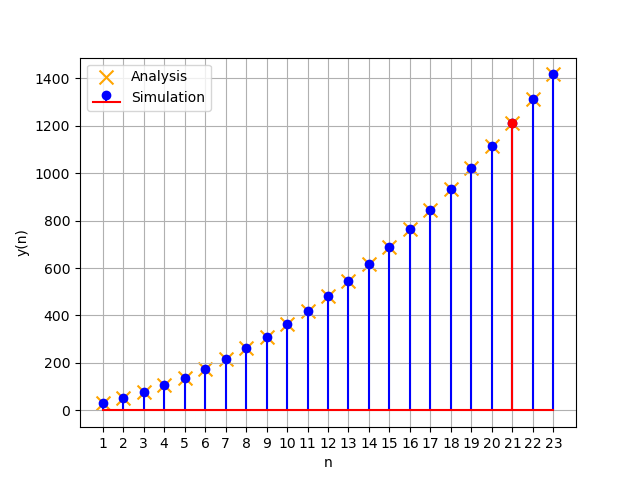
\includegraphics[scale=0.70]{./figs/fig1.png}
    \caption{ }
    \label{fig:x(n) & y(n) }
\end{figure}


\end{document}


\item Check whether -150 is a term of the AP: 11,8,5,2,....

 \solution
 \iffalse
\let\negmedspace\undefined
\let\negthickspace\undefined
\documentclass[journal,12pt,onecolumn]{IEEEtran}
\usepackage{cite}
\usepackage{amsmath,amssymb,amsfonts,amsthm}
\usepackage{algorithmic}
\usepackage{graphicx}
\usepackage{textcomp}
\usepackage{xcolor}
\usepackage{txfonts}
\usepackage{listings}
\usepackage{enumitem}
\usepackage{mathtools}
\usepackage{gensymb}
\usepackage{comment}
\usepackage[breaklinks=true]{hyperref}
\usepackage{tkz-euclide} % loads  TikZ and tkz-base
\usepackage{listings}
\usepackage[latin1]{inputenc}                                
\usepackage{color}                                            
\usepackage{array}                                            
\usepackage{longtable}                                       
\usepackage{calc}                                             
\usepackage{multirow}                                         
\usepackage{hhline}                                           
\usepackage{ifthen}                                           
\usepackage{lscape}
\usepackage{caption}


\newtheorem{theorem}{Theorem}[section]
\newtheorem{problem}{Problem}
\newtheorem{proposition}{Proposition}[section]
\newtheorem{lemma}{Lemma}[section]
\newtheorem{corollary}[theorem]{Corollary}
\newtheorem{example}{Example}[section]
\newtheorem{definition}[problem]{Definition}
%\newtheorem{thm}{Theorem}[section] 
%\newtheorem{defn}[thm]{Definition}
%\newtheorem{algorithm}{Algorithm}[section]
%\newtheorem{cor}{Corollary}
\newcommand{\BEQA}{\begin{eqnarray}}
\newcommand{\EEQA}{\end{eqnarray}}
\newcommand{\define}{\stackrel{\triangle}{=}}
\theoremstyle{remark}
\newtheorem{rem}{Remark}
%\bibliographystyle{ieeetr}

\begin{document}

%
\providecommand{\pr}[1]{\ensuremath{\Pr\left(#1\right)}}
\providecommand{\prt}[2]{\ensuremath{p_{#1}^{\left(#2\right)} }}        % own macro for this question
\providecommand{\qfunc}[1]{\ensuremath{Q\left(#1\right)}}
\providecommand{\sbrak}[1]{\ensuremath{{}\left[#1\right]}}
\providecommand{\lsbrak}[1]{\ensuremath{{}\left[#1\right.}}
\providecommand{\rsbrak}[1]{\ensuremath{{}\left.#1\right]}}
\providecommand{\brak}[1]{\ensuremath{\left(#1\right)}}
\providecommand{\lbrak}[1]{\ensuremath{\left(#1\right.}}
\providecommand{\rbrak}[1]{\ensuremath{\left.#1\right)}}
\providecommand{\cbrak}[1]{\ensuremath{\left\{#1\right\}}}
\providecommand{\lcbrak}[1]{\ensuremath{\left\{#1\right.}}
\providecommand{\rcbrak}[1]{\ensuremath{\left.#1\right\}}}
\newcommand{\sgn}{\mathop{\mathrm{sgn}}}
\providecommand{\abs}[1]{\left\vert#1\right\vert}
\providecommand{\res}[1]{\Res\displaylimits_{#1}} 
\providecommand{\norm}[1]{\left\lVert#1\right\rVert}
%\providecommand{\norm}[1]{\lVert#1\rVert}
\providecommand{\mtx}[1]{\mathbf{#1}}
\providecommand{\mean}[1]{E\left[ #1 \right]}
\providecommand{\cond}[2]{#1\middle|#2}
\providecommand{\fourier}{\overset{\mathcal{F}}{ \rightleftharpoons}}
\newenvironment{amatrix}[1]{%
  \left(\begin{array}{@{}*{#1}{c}|c@{}}
}{%
  \end{array}\right)
}
%\providecommand{\hilbert}{\overset{\mathcal{H}}{ \rightleftharpoons}}
%\providecommand{\system}{\overset{\mathcal{H}}{ \longleftrightarrow}}
        %\newcommand{\solution}[2]{\textbf{Solution:}{#1}}
\newcommand{\solution}{\noindent \textbf{Solution: }}
\newcommand{\cosec}{\,\text{cosec}\,}
\providecommand{\dec}[2]{\ensuremath{\overset{#1}{\underset{#2}{\gtrless}}}}
\newcommand{\myvec}[1]{\ensuremath{\begin{pmatrix}#1\end{pmatrix}}}
\newcommand{\mydet}[1]{\ensuremath{\begin{vmatrix}#1\end{vmatrix}}}
\newcommand{\myaugvec}[2]{\ensuremath{\begin{amatrix}{#1}#2\end{amatrix}}}
\providecommand{\rank}{\text{rank}}
\providecommand{\pr}[1]{\ensuremath{\Pr\left(#1\right)}}
\providecommand{\qfunc}[1]{\ensuremath{Q\left(#1\right)}}
        \newcommand*{\permcomb}[4][0mu]{{{}^{#3}\mkern#1#2_{#4}}}
\newcommand*{\perm}[1][-3mu]{\permcomb[#1]{P}}
\newcommand*{\comb}[1][-1mu]{\permcomb[#1]{C}}
\providecommand{\qfunc}[1]{\ensuremath{Q\left(#1\right)}}
\providecommand{\gauss}[2]{\mathcal{N}\ensuremath{\left(#1,#2\right)}}
\providecommand{\diff}[2]{\ensuremath{\frac{d{#1}}{d{#2}}}}
\providecommand{\myceil}[1]{\left \lceil #1 \right \rceil }
\newcommand\figref{Fig.~\ref}
\newcommand\tabref{Table~\ref}
\newcommand{\sinc}{\,\text{sinc}\,}
\newcommand{\rect}{\,\text{rect}\,}
%%
%       %\newcommand{\solution}[2]{\textbf{Solution:}{#1}}
%\newcommand{\solution}{\noindent \textbf{Solution: }}
%\newcommand{\cosec}{\,\text{cosec}\,}
%\numberwithin{equation}{section}
%\numberwithin{equation}{subsection}
%\numberwithin{problem}{section}
%\numberwithin{definition}{section}
%\makeatletter
%\@addtoreset{figure}{problem}
%\makeatother

%\let\StandardTheFigure\thefigure
\let\vec\mathbf

\bibliographystyle{IEEEtran}

\vspace{3cm}
\title{Assignment}
\author{EE23BTECH11001 - Aashna Sahu}
\maketitle
\bigskip

\renewcommand{\thefigure}{\theenumi}
\renewcommand{\thetable}{\theenumi}
%\renewcommand{\theequation}{\theenumi}
Q:Check whether -150 is a term of the AP: 11,8,5,2,....

 \solution
 \fi

\begin{align}
x(n)&=x(0)+nd\\
n&=\frac{x(n)-x(0)}{d}
\end{align}
\begin{align}
x(n)-x(0) &\equiv 0 \pmod{d}
\end{align}
On substitutings values\\
\begin{align}
-161 &\equiv 2 \pmod{-3}
\end{align}
Thus -150 is not a term of the given AP.
\begin{align}
 \boxed{x(n)=(11-3n)\times u(n)}   
\end{align}

\begin{align}
   X(z)&=\frac{11}{1-z^{-1}}-\frac{3z^{-1}}{(1-z^{-1})^2}\quad
    |z|>1
\end{align}

    \begin{table}[h]
    \centering
    
        \begin{tabular}{|c|c|c|}
      \hline
      Variable & Description & Value\\\hline
      $x(0)$ & First term of AP & 11\\\hline
      $d$ & Common difference & -3\\\hline
      $x(n)$ & General term of given AP & None\\\hline
      \end{tabular}

        
    \caption{Input parameters}
    \label{tab:Table1}
\end{table}
\newpage
\begin{figure}[h]
  \centering
  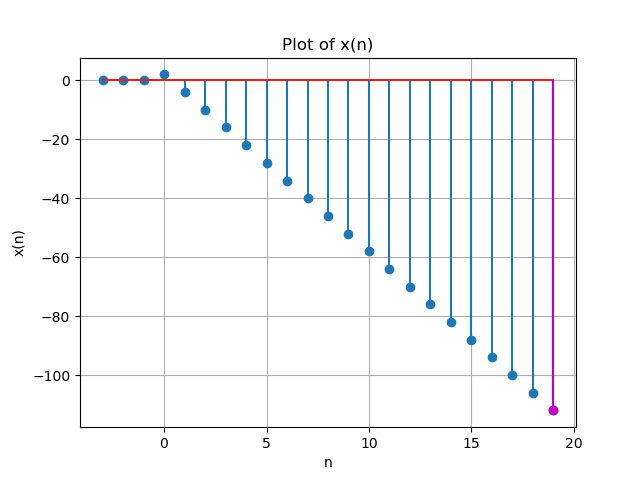
\includegraphics[width=1.2\columnwidth]{figs/Figure_1.png}
  \captionsetup {justification=centering}
  \caption{Representation of x(n)}
  \label{fig:fig1}
\end{figure}
%\end{document}

 

 \item Write the first five terms of the sequence \(a_n = \frac{n(n^2+5)}{4}\).

\solution
\iffalse
\let\negmedspace\undefined
\let\negthickspace\undefined
\documentclass[journal,12pt,onecolumn]{IEEEtran}
\usepackage{cite}
\usepackage{amsmath,amssymb,amsfonts,amsthm}
\usepackage{algorithmic}
\usepackage{graphicx}
\usepackage{textcomp}
\usepackage{xcolor}
\usepackage{txfonts}
\usepackage{listings}
\usepackage{enumitem}
\usepackage{mathtools}
\usepackage{gensymb}

\usepackage{tkz-euclide} % loads  TikZ and tkz-base
\usepackage{listings}



\newtheorem{theorem}{Theorem}[section]
\newtheorem{problem}{Problem}
\newtheorem{proposition}{Proposition}[section]
\newtheorem{lemma}{Lemma}[section]
\newtheorem{corollary}[theorem]{Corollary}
\newtheorem{example}{Example}[section]
\newtheorem{definition}[problem]{Definition}
%\newtheorem{thm}{Theorem}[section] 
%\newtheorem{defn}[thm]{Definition}
%\newtheorem{algorithm}{Algorithm}[section]
%\newtheorem{cor}{Corollary}
\newcommand{\BEQA}{\begin{eqnarray}}
\newcommand{\EEQA}{\end{eqnarray}}
\newcommand{\system}[1]{\stackrel{#1}{\rightarrow}}

\newcommand{\define}{\stackrel{\triangle}{=}}
\theoremstyle{remark}
\newtheorem{rem}{Remark}
%\bibliographystyle{ieeetr}
\begin{document}
%
\providecommand{\pr}[1]{\ensuremath{\Pr\left(#1\right)}}
\providecommand{\prt}[2]{\ensuremath{p_{#1}^{\left(#2\right)} }}        % own macro for this question
\providecommand{\qfunc}[1]{\ensuremath{Q\left(#1\right)}}
\providecommand{\sbrak}[1]{\ensuremath{{}\left[#1\right]}}
\providecommand{\lsbrak}[1]{\ensuremath{{}\left[#1\right.}}
\providecommand{\rsbrak}[1]{\ensuremath{{}\left.#1\right]}}
\providecommand{\brak}[1]{\ensuremath{\left(#1\right)}}
\providecommand{\lbrak}[1]{\ensuremath{\left(#1\right.}}
\providecommand{\rbrak}[1]{\ensuremath{\left.#1\right)}}
\providecommand{\cbrak}[1]{\ensuremath{\left\{#1\right\}}}
\providecommand{\lcbrak}[1]{\ensuremath{\left\{#1\right.}}
\providecommand{\rcbrak}[1]{\ensuremath{\left.#1\right\}}}
\newcommand{\sgn}{\mathop{\mathrm{sgn}}}
\providecommand{\abs}[1]{\left\vert#1\right\vert}
\providecommand{\res}[1]{\Res\displaylimits_{#1}} 
\providecommand{\norm}[1]{\left\lVert#1\right\rVert}
%\providecommand{\norm}[1]{\lVert#1\rVert}
\providecommand{\mtx}[1]{\mathbf{#1}}
\providecommand{\mean}[1]{E\left[ #1 \right]}
\providecommand{\cond}[2]{#1\middle|#2}
\providecommand{\fourier}{\overset{\mathcal{F}}{ \rightleftharpoons}}
\newenvironment{amatrix}[1]{%
  \left(\begin{array}{@{}*{#1}{c}|c@{}}
}{%
  \end{array}\right)
}
%\providecommand{\hilbert}{\overset{\mathcal{H}}{ \rightleftharpoons}}
%\providecommand{\system}{\overset{\mathcal{H}}{ \longleftrightarrow}}
	%\newcommand{\solution}[2]{\textbf{Solution:}{#1}}
\newcommand{\solution}{\noindent \textbf{Solution: }}
\newcommand{\cosec}{\,\text{cosec}\,}
\providecommand{\dec}[2]{\ensuremath{\overset{#1}{\underset{#2}{\gtrless}}}}
\newcommand{\myvec}[1]{\ensuremath{\begin{pmatrix}#1\end{pmatrix}}}
\newcommand{\mydet}[1]{\ensuremath{\begin{vmatrix}#1\end{vmatrix}}}
\newcommand{\myaugvec}[2]{\ensuremath{\begin{amatrix}{#1}#2\end{amatrix}}}
\providecommand{\rank}{\text{rank}}
\providecommand{\pr}[1]{\ensuremath{\Pr\left(#1\right)}}
\providecommand{\qfunc}[1]{\ensuremath{Q\left(#1\right)}}
	\newcommand*{\permcomb}[4][0mu]{{{}^{#3}\mkern#1#2_{#4}}}
\newcommand*{\perm}[1][-3mu]{\permcomb[#1]{P}}
\newcommand*{\comb}[1][-1mu]{\permcomb[#1]{C}}
\providecommand{\qfunc}[1]{\ensuremath{Q\left(#1\right)}}
\providecommand{\gauss}[2]{\mathcal{N}\ensuremath{\left(#1,#2\right)}}
\providecommand{\diff}[2]{\ensuremath{\frac{d{#1}}{d{#2}}}}
\providecommand{\myceil}[1]{\left \lceil #1 \right \rceil }
\newcommand\figref{Fig.~\ref}
\newcommand\tabref{Table~\ref}
\newcommand{\sinc}{\,\text{sinc}\,}
\newcommand{\rect}{\,\text{rect}\,}
%%
%	%\newcommand{\solution}[2]{\textbf{Solution:}{#1}}
%\newcommand{\solution}{\noindent \textbf{Solution: }}
%\newcommand{\cosec}{\,\text{cosec}\,}
%\numberwithin{equation}{section}
%\numberwithin{equation}{subsection}
%\numberwithin{problem}{section}
%\numberwithin{definition}{section}
%\makeatletter
%\@addtoreset{figure}{problem}
%\makeatother

%\let\StandardTheFigure\thefigure
\let\vec\mathbf

\bibliographystyle{IEEEtran}





\bigskip

\renewcommand{\thefigure}{\theenumi}
\renewcommand{\thetable}{\theenumi}
%\renewcommand{\theequation}{\theenumi}


\title{Discrete Assignment}
\author{Karyampudi Meghana Sai\\ EE23BTECH11031}
\maketitle


Write the first five terms of the sequence \(a_n = \frac{n(n^2+5)}{4}\).

\solution
\fi
\begin{align}
 x(n) &= \left(\frac{n^3+3n^2+8n+6}{4}\right) u(n)\label{eq:1}
\end{align}
\begin{align}
 n^k u(n) \system{Z} (-1)^k z^k \frac{d^k}{dz^k}U(z)
\end{align}

\begin{align}
    nu(n) &\system{Z} \frac{z^{-1}}{(1 - z^{-1})^2} \quad \abs{ z} > 1  \label{eq:3} \\
    n^2u(n) &\system{Z} \frac{(z^{-1})(1+z^{-1})}{(1 - z^{-1})^3} \quad \abs{ z} > 1  \label{eq:4} \\
    n^3u(n) &\system{Z} \frac{(z^{-1})(1+4z^{-1}+z^{-2})}{(1 - z^{-1})^4} \quad \abs{ z} > 1  \label{eq:5} 
\end{align}
Referencing the equations from \eqref{eq:3}, \eqref{eq:4}, and \eqref{eq:5}.
\begin{align}
    x(n) &\system{Z} \frac{(z^{-1})(1+4z^{-1}+z^{-2})}{4(1-z^{-1})^4} + \frac{3(z^{-1})(1+z^{-1})}{4(1-z^{-1})^3} + \frac{2z^{-1}}{(1 - z^{-1})^2} + \frac{3}{2(1- z^{-1})} \quad \abs{ z} > 1  \label{eq:6} \\
    x(n) &\system{Z} \frac{3}{2(1-z^{-1})^3} + \frac{3z^{-2}}{2(1-z^{-1})^4}\quad \abs{ z} > 1  \label{eq:} 
\end{align}

\begin{figure}[h]
    \centering
    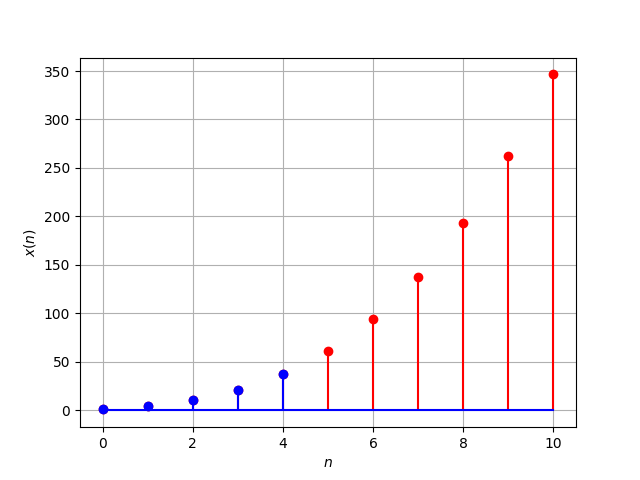
\includegraphics[width=\columnwidth]{ncert-maths/11/9/1/6/figs/plot_from_c.png}
    \caption{Plot of equation\eqref{eq:1}}
    \label{fig:}
\end{figure}
%\end{document}




\item
\begin{enumerate}
\item 30th term of the AP: 10, 7, 4, $\ldots$ is 
\item 11th term of the AP: $-3, -\frac{1}{2}, 2, \ldots$ is
\end{enumerate}
\solution
\iffalse
\let\negmedspace\undefined
\let\negthickspace\undefined
\documentclass[journal,12pt,twocolumn]{IEEEtran}
\usepackage{cite}
\usepackage{amsmath,amssymb,amsfonts,amsthm}
\usepackage{algorithmic}
\usepackage{graphicx}
\usepackage{textcomp}
\usepackage{xcolor}
\usepackage{txfonts}
\usepackage{listings}
\usepackage{enumitem}
\usepackage{mathtools}
\usepackage{gensymb}
\usepackage{comment}
\usepackage[breaklinks=true]{hyperref}
\usepackage{tkz-euclide}
\usepackage{listings}
\usepackage{gvv}
\def\inputGnumericTable{}
\usepackage[latin1]{inputenc}
\usepackage{color}
\usepackage{array}
\usepackage{longtable}
\usepackage{calc}
\usepackage{multirow}
\usepackage{hhline}
\usepackage{ifthen}
\usepackage{lscape}

\newtheorem{theorem}{Theorem}[section]
\newtheorem{problem}{Problem}
\newtheorem{proposition}{Proposition}[section]
\newtheorem{lemma}{Lemma}[section]
\newtheorem{corollary}[theorem]{Corollary}
\newtheorem{example}{Example}[section]
\newtheorem{definition}[problem]{Definition}
\newcommand{\BEQA}{\begin{eqnarray}}
\newcommand{\EEQA}{\end{eqnarray}}
\newcommand{\define}{\stackrel{\triangle}{=}}
\theoremstyle{remark}
\newtheorem{rem}{Remark}
\begin{document}

\bibliographystyle{IEEEtran}
\vspace{3cm}

\title{NCERT Discrete - 10.5.2.2}
\author{EE23BTECH11058 - Sindam Ananya$^{*}$% <-this % stops a space
}
\maketitle
\newpage
\bigskip

\renewcommand{\thefigure}{\theenumi}
\renewcommand{\thetable}{\theenumi}

\vspace{3cm}
\textbf{Question 10.5.2.2:} 
\begin{enumerate}
\item 30th term of the AP: 10, 7, 4, $\ldots$ is 
\item 11th term of the AP: $-3, -\frac{1}{2}, 2, \ldots$ is
\end{enumerate}
\solution
\fi
\begin{table}[h!]
    \centering
    \begin{tabular}{ | c | c | c | }
        \hline
        \textbf{Parameter}  & \textbf{value} & \textbf{Description} \\
        \hline
        \multirow{2}{*}{\begin{tabular}[c]{@{}c@{}}$x_i(0)$\\  \end{tabular}} & 10 & \multirow{2}{*}{\begin{tabular}[c]{@{}c@{}}First \\ term\end{tabular}} \\
        \cline{2-2}
        & -3 &  \\
        \hline
        \multirow{2}{*}{\begin{tabular}[c]{@{}c@{}}$d_i$ \\ \end{tabular}} & -3 & \multirow{2}{*}{\begin{tabular}[c]{@{}c@{}}Common \\ difference\end{tabular}} \\
        \cline{2-2}
          & $\frac{5}{2}$ &  \\
        \hline
        $x_1(29)$ &  ? & 30th term \\
        \hline
        $x_2(10)$ & ? & 11th term \\
        \hline
    \end{tabular}

    \caption{Input Parameters}
    \label{tab:table1}
    \end{table}
\begin{equation}
    x_i(n) = \sbrak{x_i(0) + nd_i} u(n)
    \label{eq:eq1}
\end{equation}
\begin{enumerate}
\item From \eqref{eq:eq1} \tabref{tab:table1} :
\begin{align}
x_1(n) &= \sbrak{10 -3n}u(n)\\
x_1(29) &= -77\\
X_1(z) &= \frac{10 - 13z^{-1}}{(1-z^{-1})^2} \quad \abs{z} > 1
\end{align}
\item From \eqref{eq:eq1} and \tabref{tab:table1} :
\begin{align}
x_2(n) &= \sbrak{-3 + \frac{5}{2}n}u(n)\\
x_2(10) &= 22\\
X_2(z) &= \frac{5.5z^{-1}-3}{(1-z^{-1})^2} \quad \abs{z}> 1
\end{align}
\end{enumerate}
\begin{figure}[h!]
    \centering
    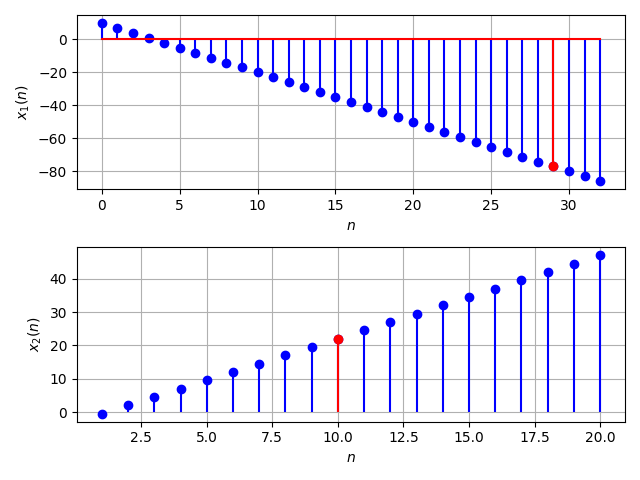
\includegraphics[width=\columnwidth]{ncert-maths/10/5/2/2/figs/plot.png}
    \caption{stem plots of $x_1(n)$ and $x_2(n)$}
    \label{fig:1}
\end{figure}
%\end{document}



\item Write the first five terms of the sequence whose nth term is $\frac{2n-3}{6}$ and obtain the Z transform of the series
\solution
\let\negmedspace\undefined
\let\negthickspace\undefined
\documentclass[journal,12pt,twocolumn]{IEEEtran}
\usepackage{cite}
\usepackage{amsmath,amssymb,amsfonts,amsthm}
\usepackage{algorithmic}
\usepackage{graphicx}
\usepackage{textcomp}
\usepackage{xcolor}
\usepackage{txfonts}
\usepackage{listings}
\usepackage{enumitem}
\usepackage{mathtools}
\usepackage{gensymb}
\usepackage{comment}
\usepackage[breaklinks=true]{hyperref}
\usepackage{tkz-euclide} 
\usepackage{listings}
\usepackage{gvv}                                        
\def\inputGnumericTable{}                                 
\usepackage[latin1]{inputenc}                                
\usepackage{color}                                            
\usepackage{array}                                            
\usepackage{longtable}                                       
\usepackage{calc}                                             
\usepackage{multirow}                                         
\usepackage{hhline}                                           
\usepackage{ifthen}                                           
\usepackage{lscape}

\newtheorem{theorem}{Theorem}[section]
\newtheorem{problem}{Problem}
\newtheorem{proposition}{Proposition}[section]
\newtheorem{lemma}{Lemma}[section]
\newtheorem{corollary}[theorem]{Corollary}
\newtheorem{example}{Example}[section]
\newtheorem{definition}[problem]{Definition}
\newcommand{\BEQA}{\begin{eqnarray}}
\newcommand{\EEQA}{\end{eqnarray}}
\newcommand{\define}{\stackrel{\triangle}{=}}
\theoremstyle{remark}
\newtheorem{rem}{Remark}

\begin{document}
\bibliographystyle{IEEEtran}

\vspace{3cm}

\title{}
\author{EE23BTECH11047 - Deepakreddy P
}
\maketitle
\newpage
\bigskip

\section*{Exercise 9.1}

\noindent \textbf{4} \quad Write the first five terms of the sequence whose nth term is $\frac{2n-3}{6}$ and obtain the Z transform of the series\\
\solution
\begin{align}
x \brak{n} &= \frac{2n-1}{6} \brak{u\brak{n}}
\label{x(n)}
\end{align}

\begin{figure}[h]
   \centering
   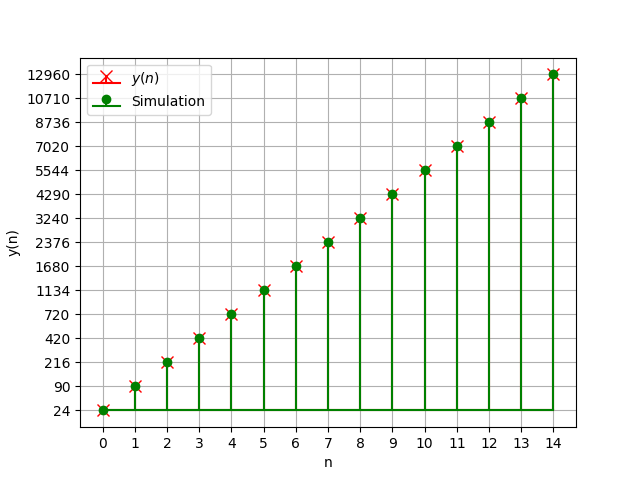
\includegraphics[width=1\columnwidth]{figs/plot.png}
   \caption{Plot of x(n) vs n}
   \label{fig: 9.1.4.1}
\end{figure}

\begin{align}
X(z) &= {\frac{3z^{-1}-1}{6(1-z^{-1})^{2}}\quad|z|>1}
\end{align}


\end{document}


 \item For what values of x, the numbers $-\frac{2}{7}\,,x,-\frac{7}{2}\,$ are in G.P ?

\solution
\iffalse
\let\negmedspace\undefined
\let\negthickspace\undefined
\documentclass[journal,12pt,twocolumn]{IEEEtran}
\usepackage{cite}
\usepackage{amsmath,amssymb,amsfonts,amsthm}
\usepackage{algorithmic}
\usepackage{graphicx}
\usepackage{textcomp}
\usepackage[justification=centering]{caption}
\usepackage{xcolor}
\usepackage{txfonts}
\usepackage{listings}
\usepackage{enumitem}
\usepackage{mathtools}
\usepackage{gensymb}
\usepackage{comment}
\usepackage[breaklinks=true]{hyperref}
\usepackage{tkz-euclide} 
\usepackage{listings}
\usepackage{gvv}                                        
\def\inputGnumericTable{}                                 
\usepackage[latin1]{inputenc}                                
\usepackage{color}                                            
\usepackage{array}                                            
\usepackage{longtable}                                       
\usepackage{calc}                                             
\usepackage{multirow}                                         
\usepackage{hhline}                                           
\usepackage{ifthen}                                           
\usepackage{lscape}

\newtheorem{theorem}{Theorem}[section]
\newtheorem{problem}{Problem}
\newtheorem{proposition}{Proposition}[section]
\newtheorem{lemma}{Lemma}[section]
\newtheorem{corollary}[theorem]{Corollary}
\newtheorem{example}{Example}[section]
\newtheorem{definition}[problem]{Definition}
\newcommand{\BEQA}{\begin{eqnarray}}
\newcommand{\EEQA}{\end{eqnarray}}
\newcommand{\define}{\stackrel{\triangle}{=}}
\theoremstyle{remark}
\newtheorem{rem}{Remark}
\begin{document}

\bibliographystyle{IEEEtran}
\vspace{3cm}

\title{11.9.3.6}
\author{EE23BTECH11022 - G DILIP REDDY}
\maketitle
\newpage

\bigskip

\renewcommand{\thefigure}{\theenumi}
\renewcommand{\thetable}{\theenumi}
\textbf{Question}:\\
For what values of x, the numbers $-\frac{2}{7}\,,x,-\frac{7}{2}\,$ are in G.P ?
\\\\
\textbf{Solution: }\\
\fi
\begin{table}[h]
    \centering
    \renewcommand\thetable{1}
    \begin{tabular}[12.1pt]{ |c| c| c|}
    \hline
    \textbf{Variable} & \textbf{Description} &\textbf{Value}\\ 
    \hline
    $x(0)$ & First term of the GP &$-\brak{\frac{2}{7}}$ \\
    \hline 
    $x(1)$ & Second term of the GP &$x$ \\
    \hline 
    $x(2)$ & Third term of the GP &$-\brak{\frac{7}{2}}$ \\
    \hline 
    $r$ & Common ratio of the GP & \\
    \hline
    $x(n)$ & General term & $x(0)\,r^n\,u(n)$\\
    \hline    
\end{tabular}

    \caption{Variables Used}
    \label{tab:table_11.9.3.6}
\end{table}
Let $r$ be the common ratio\\
From \tabref{tab:table_11.9.3.6}:
\begin{align}
\implies \frac{x}{\brak{-\frac{2}{7}\,}}\,&= \frac{\brak{-\frac{7}{2}\,}}{x}\,=r \\
x^2&=\brak{-\frac{2}{7}\,}\cdot\brak{-\frac{7}{2}\,}\\
x&=\pm 1\\
\implies r&=\pm \frac{7}{2}\,\\\notag
\end{align}
The signal corresponding to this is 
\begin{align}
x(n)=\brak{-\frac{2}{7}}\brak{\pm \frac{7}{2}}^n\,u(n)
\end{align}
Applying z-Transform :
\begin{align}
\implies X_1(z)&=\brak{\frac{1}{7}}\brak{\frac{4}{7z^{-1}+2}\,}
\quad \abs{z}>\frac{7}{2}\\
\implies X_2(z)&=\brak{\frac{1}{7}}\brak{\frac{4}{7z^{-1}-2}\,}
\quad \abs{z}>\frac{7}{2}
\end{align}
\begin{figure}[h]
    \renewcommand\thefigure{1}
    \centering
    \captionsetup{justification=centering}
    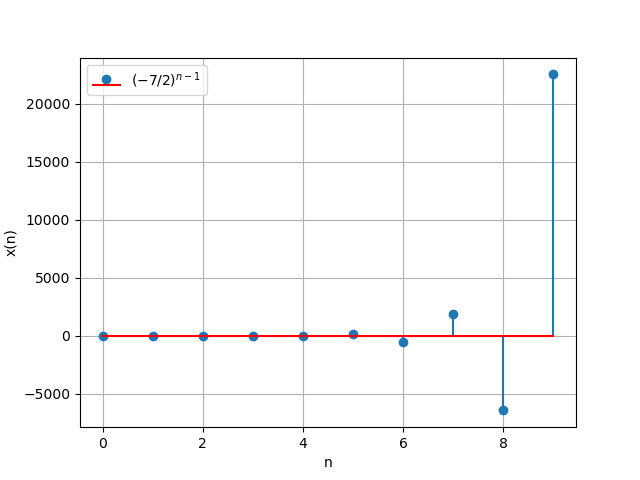
\includegraphics[width=1.1\linewidth]{ncert-maths/11/9/3/6/figs/graph1.png}
    \caption{Stem Plot of $x_1$(n)}
    \label{stemplot1}
\end{figure}
\begin{figure}[h]
    \renewcommand\thefigure{2}
    \centering
    \captionsetup{justification=centering}
    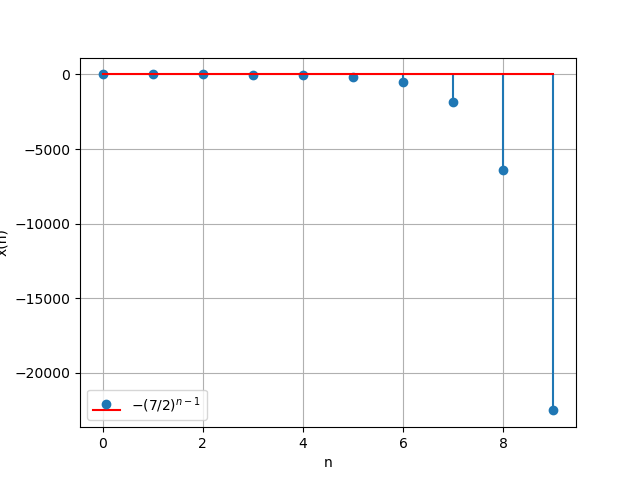
\includegraphics[width=1.1\linewidth]{ncert-maths/11/9/3/6/figs/graph2.png}
    \caption{Stem Plot of $x_2(n)$}
    \label{stemplot2}
\end{figure}
%\end{document}



\item Find the $20^{th}$ and $n^{th}$ terms of the G.P $\frac{5}{2}$, $\frac{5}{4}$, $\frac{5}{8}$,.....

\solution
 \iffalse
\let\negmedspace\undefined
\let\negthickspace\undefined
\documentclass[journal,12pt,twocolumn]{IEEEtran}
\usepackage{cite}
\usepackage{amsmath,amssymb,amsfonts,amsthm}
\usepackage{algorithmic}
\usepackage{graphicx}
\usepackage{textcomp}
\usepackage{xcolor}
\usepackage{txfonts}
\usepackage{listings}
\usepackage{enumitem}
\usepackage{mathtools}
\usepackage{gensymb}
\usepackage{comment}
\usepackage[breaklinks=true]{hyperref}
\usepackage{tkz-euclide} 
\usepackage{listings}
\usepackage{gvv}                                        
\def\inputGnumericTable{}                                 
\usepackage[latin1]{inputenc}                                
\usepackage{color}                                            
\usepackage{array}                                            
\usepackage{longtable}                                       
\usepackage{calc}                                             
\usepackage{multirow}                                         
\usepackage{hhline}                                           
\usepackage{ifthen}                                           
\usepackage{lscape}
\usepackage{caption}
\newtheorem{theorem}{Theorem}[section]
\newtheorem{problem}{Problem}
\newtheorem{proposition}{Proposition}[section]
\newtheorem{lemma}{Lemma}[section]
\newtheorem{corollary}[theorem]{Corollary}
\newtheorem{example}{Example}[section]
\newtheorem{definition}[problem]{Definition}
\newcommand{\BEQA}{\begin{eqnarray}}
\newcommand{\EEQA}{\end{eqnarray}}
\newcommand{\define}{\stackrel{\triangle}{=}}
\theoremstyle{remark}
\newtheorem{rem}{Remark}
\begin{document}
\parindent 0px
\bibliographystyle{IEEEtran}
\vspace{3cm}

\title{NCERT 11.9.3 1Q}
\author{EE23BTECH11013 - Avyaaz$^{*}$% <-this % stops a space
}
\maketitle
\newpage
\bigskip

\renewcommand{\thefigure}{\arabic{figure}}
\renewcommand{\thetable}{\arabic{table}}
\large\textbf{\textsl{Question:}}
Find the $20^{th}$ and $n^{th}$ terms of the G.P $\frac{5}{2}$, $\frac{5}{4}$, $\frac{5}{8}$,.....

\solution
\fi
 \begin{table}[htbp]
     \centering
     \setlength{\extrarowheight}{8pt}
    \begin{table}[ht]
    \centering
    \begin{tabular}{|c|c|c|}
        \hline
        Parameter & Value & Description \\
        \hline
        $x(0)$ & 5 & First term of AP \\
        $d$ & 1.75 & Common difference of AP \\
        $x(n)$ & 20.75 & $n^{th}$ term of AP \\
        \hline
    \end{tabular}
    \vspace{2mm}
    \caption{Parameter List}
    \label{tab:simple.10.5.2.20}
\end{table}

     \caption{Parameters}
     \label{tab:table1}
 \end{table} 

% \begin{align}
%    x(n) = \dfrac{5}{2}\left(\dfrac{1}{2}\right)^n 
% \end{align}

% \begin{align}
% 	x \brak{n} & \system{Z} X \brak{z} \\
%    % x(n) &=\dfrac{5}{2}\left(\dfrac{1}{2}\right)^n u(n) \\
%     \therefore X(z) &= \sum_{n=-\infty}^{\infty}x(n)z^{-n}\label{eq:z-transform}  
% \end{align}
% Here, 
%          $    u(n) = \begin{cases}
%                 0 &\text{for } n < 0 \\
%                 1 & \text{for } n \geq 0
%             \end{cases}$       
 
%  \vspace{1cm}
From \tabref{tab:table1}:
\(Z\)-Transform of \(x(n)\):
\begin{align}
% \implies X(z) &= \sum_{n=-\infty}^{\infty}\left(\dfrac{5}{2}\left(\dfrac{1}{2}\right)^n u(n)\right) z^{-n} \\
 % \implies X(z) &= \dfrac{5}{2}\sum_{n=0}^{\infty}\left(\dfrac{z
 % ^{-1}}{2}\right)^n \\
\implies X(z) &=\dfrac{5}{2}\left(\dfrac{1}{1-\frac{z^{-1}}{2}}\right) ;\cbrak{z\in\mathbb{C} : |z|>\dfrac{1}{2}}
\end{align}

\begin{figure}[ht]
    \centering
    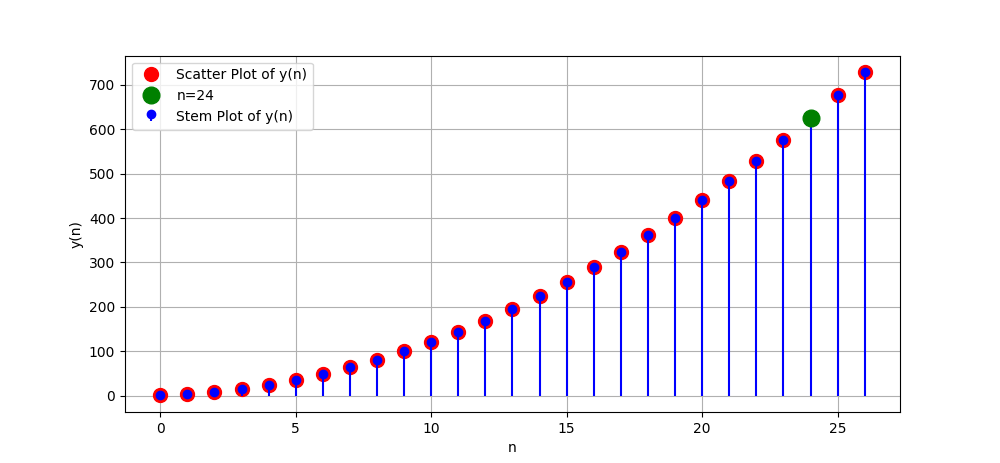
\includegraphics[width = \columnwidth]{figs/stem_plot.png}
    \caption{}
    \label{fig:graph1}
\end{figure} 

\bibliographystyle{IEEEtran}
%\end{document}



\item 
Which term of the following sequences:\\
(a) 2,$2\sqrt{2}$,4\dots is 128
\quad(b) $\sqrt{3}$,3,$3\sqrt{3}$\dots is 729\\
(c) $\frac{1}{3}$,$\frac{1}{9}$,$\frac{1}{27}$\dots is $\frac{1}{19683}$ \\
\solution
\iffalse
\let\negmedspace\undefined
\let\negthickspace\undefined
\documentclass[journal,12pt,twocolumn]{IEEEtran}
\usepackage{cite}
\usepackage{amsmath,amssymb,amsfonts,amsthm}
\usepackage{algorithmic}
\usepackage{graphicx}
\usepackage{textcomp}
\usepackage{xcolor}
\usepackage{txfonts}
\usepackage{listings}
\usepackage{enumitem}
\usepackage{mathtools}
\usepackage{gensymb}
\usepackage{comment}
\usepackage[breaklinks=true]{hyperref}
\usepackage{tkz-euclide} 
\usepackage{listings}
\usepackage{gvv}                                        
\def\inputGnumericTable{}                                 
\usepackage[latin1]{inputenc}                                
\usepackage{color}                                            
\usepackage{array}                                            
\usepackage{longtable}                                       
\usepackage{calc}                                             
\usepackage{multirow}                                         
\usepackage{hhline}                                           
\usepackage{ifthen}                                           
\usepackage{lscape}
\usepackage[center]{caption} % center the captions to figure

\newtheorem{theorem}{Theorem}[section]
\newtheorem{problem}{Problem}
\newtheorem{proposition}{Proposition}[section]
\newtheorem{lemma}{Lemma}[section]
\newtheorem{corollary}[theorem]{Corollary}
\newtheorem{example}{Example}[section]
\newtheorem{definition}[problem]{Definition}
\newcommand{\BEQA}{\begin{eqnarray}}
\newcommand{\EEQA}{\end{eqnarray}}
\newcommand{\define}{\stackrel{\triangle}{=}}
\theoremstyle{remark}
\newtheorem{rem}{Remark}
\begin{document}

\newcolumntype{M}[1]{>{\centering\arraybackslash}m{#1}}
\newcolumntype{N}{@{}m{0pt}@{}}

\bibliographystyle{IEEEtran}
\vspace{3cm}

\title{NCERT 11.9.3 5Q} 
\author{ee23btech11223 - Soham Prabhakar More% <-this % stops a space
}
\maketitle
\newpage
\bigskip

\renewcommand{\thefigure}{\theenumi}
\renewcommand{\thetable}{\theenumi}

\bibliographystyle{IEEEtran}

\textbf{Question:}\\
Which term of the following sequences:\\
(a) 2,$2\sqrt{2}$,4\dots is 128
\quad(b) $\sqrt{3}$,3,$3\sqrt{3}$\dots is 729\\
(c) $\frac{1}{3}$,$\frac{1}{9}$,$\frac{1}{27}$\dots is $\frac{1}{19683}$
\fi 
For a general GP series and $k > 0$,
\begin{align}
    x\brak{k} &= x\brak{0}r^k \\
    \therefore k &= \log_r{\frac{x\brak{k}}{x\brak{0}}} \label{eq:gsoln}
\end{align}
And the Z-transform $X\brak{z}$:
\begin{align}
    X\brak{z} &= \frac{x\brak{0}}{1 - rz^{-1}} \quad {\abs{z} > \abs{r}} \label{eq:zresult}
\end{align}

\begin{enumerate}[label=(\alph*)]
\item By \tabref{Table:1}, \eqref{eq:gsoln} and \tabref{Table:1}: % prob:a
\begin{align}
    x_1\brak{n} &= x_1\brak{0} r_1^nu\brak{n} \\
    k_1 &= \log_{r_1}{\frac{128}{x_1\brak{0}}} \\
    \therefore k_1 &= 12 \\
	X_1\brak{z} &= \frac{2}{1 - \sqrt{2}z^{-1}} \quad \abs{z} > \sqrt{2}
\end{align}

\begin{figure}[h!]
    \renewcommand\thefigure{1}
    \centering
    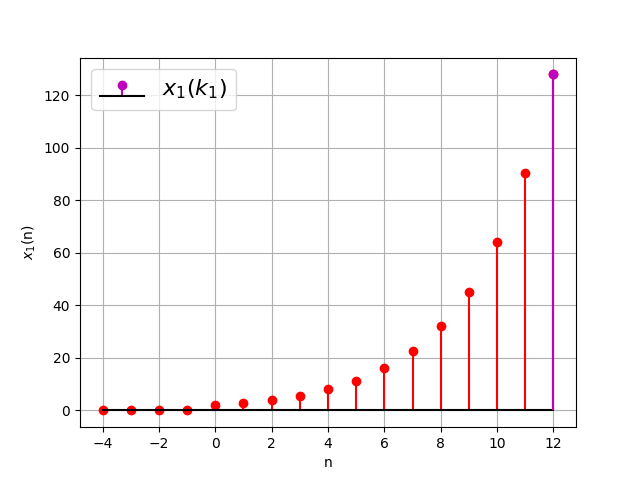
\includegraphics[width=\columnwidth]{ncert-maths/11/9/3/5/figs/a.png}
    \caption[short]{Plot of $x_1$\brak{n} vs n. See \tabref{Table:1}}
    \label{fig:img1}
\end{figure}



\item By \eqref{eq:gsoln}, \eqref{eq:zresult} and \tabref{Table:1}: % prob:b
\begin{align}
    x_2\brak{n} &= x_2\brak{0} r_2^nu\brak{n} \\
    k_2 &= \log_{r_2}{\frac{729}{x_2\brak{0}}} \\
    \therefore k_2 &= 11 \\
    X_2\brak{z} &= \frac{\sqrt{3}}{1 - \sqrt{3}z^{-1}} \quad \abs{z} > \sqrt{3} 
\end{align}

\begin{figure}[h!]
    \renewcommand\thefigure{2}
    \centering
    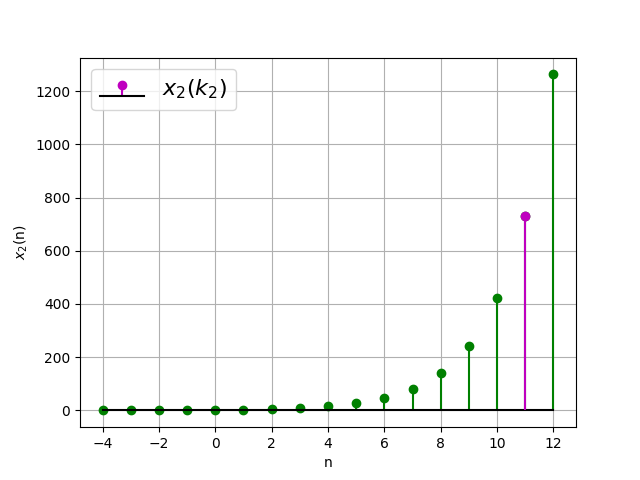
\includegraphics[width=\columnwidth]{ncert-maths/11/9/3/5/figs/b.png}
    \caption[short]{Plot of $x_2$\brak{n} vs n. See \tabref{Table:1}}
    \label{fig:img2}
\end{figure}

\item By \eqref{eq:gsoln}, \eqref{eq:zresult} and \tabref{Table:1}: % prob:c
\begin{align}
    x_3\brak{n} &= x_3\brak{0} r_3^nu\brak{n} \\
    k_3 &= \log_{r_3}{\frac{1}{19683 x_3\brak{0}}} \\
    \therefore k_3 &= 8 \\
    X_3\brak{z} &= \frac{1}{3 - z^{-1}} \quad \abs{z} > \frac{1}{3}
\end{align}

\begin{figure}[h!]
    \renewcommand\thefigure{3}
    \centering
    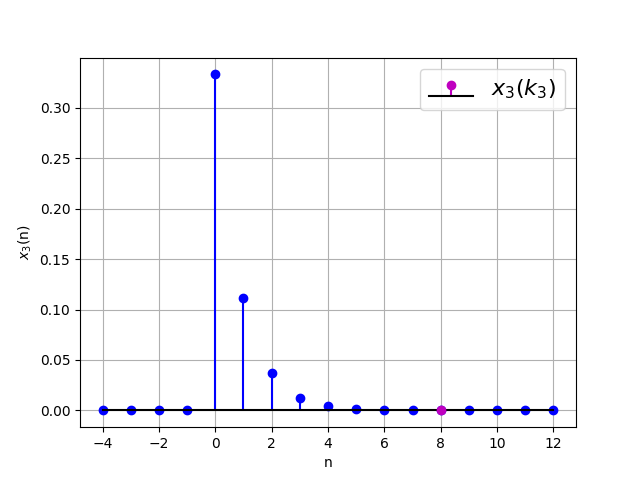
\includegraphics[width=\columnwidth]{ncert-maths/11/9/3/5/figs/c.png}
    \caption[short]{Plot of $x_3$\brak{n} vs n. See \tabref{Table:1}}
    \label{fig:img3}
\end{figure}

\begin{table}[ht]
\begin{tabular}{|c|c|c|}
    \hline 
    \textbf{Parameter}&\textbf{Description} &\textbf{Value}\\
    \hline 
    $r_i$ & Common ratio of G.P (a),(b),(c) & $\sqrt{2}, \sqrt{3}, \frac{1}{3}$ \\
    \hline
    $x_i(0)$ & Initial Values & $2, \sqrt{3}, \frac{1}{3}$ \\
    \hline
    $x_i(k_i)$ & Given Values & $128, 729, \frac{1}{19683}$ \\
    \hline 
    $k_i$ & Desired index & $12, 11, 8$ \\
    \hline 
    $x_i\brak{n}$ & Series & $x_i\brak{0}r_i^nu\brak{n}$ \\
    \hline
	$X_i\brak{z}$ & Z-Transform of $x_i\brak{n}$ & $\frac{x\brak{0}}{1-rz^{-1}}$ \\
    \hline
\end{tabular}

\caption{Table of parameters}
\label{Table:1}


\end{table}

\end{enumerate}

Find the $20^{th}$ and $n^{th}$ terms of the G.P $\frac{5}{2}$, $\frac{5}{4}$, $\frac{5}{8}$,.....

% \item 
% Which term of the following sequences:\\
% (a) 2,$2\sqrt{2}$,4\dots is 128
% \quad(b) $\sqrt{3}$,3,$3\sqrt{3}$\dots is 729\\
% (c) $\frac{1}{3}$,$\frac{1}{9}$,$\frac{1}{27}$\dots is $\frac{1}{19683}$
% \solution
% \iffalse
\let\negmedspace\undefined
\let\negthickspace\undefined
\documentclass[journal,12pt,twocolumn]{IEEEtran}
\usepackage{cite}
\usepackage{amsmath,amssymb,amsfonts,amsthm}
\usepackage{algorithmic}
\usepackage{graphicx}
\usepackage{textcomp}
\usepackage{xcolor}
\usepackage{txfonts}
\usepackage{listings}
\usepackage{enumitem}
\usepackage{mathtools}
\usepackage{gensymb}
\usepackage{comment}
\usepackage[breaklinks=true]{hyperref}
\usepackage{tkz-euclide} 
\usepackage{listings}
\usepackage{gvv}                                        
\def\inputGnumericTable{}                                 
\usepackage[latin1]{inputenc}                                
\usepackage{color}                                            
\usepackage{array}                                            
\usepackage{longtable}                                       
\usepackage{calc}                                             
\usepackage{multirow}                                         
\usepackage{hhline}                                           
\usepackage{ifthen}                                           
\usepackage{lscape}
\usepackage[center]{caption} % center the captions to figure

\newtheorem{theorem}{Theorem}[section]
\newtheorem{problem}{Problem}
\newtheorem{proposition}{Proposition}[section]
\newtheorem{lemma}{Lemma}[section]
\newtheorem{corollary}[theorem]{Corollary}
\newtheorem{example}{Example}[section]
\newtheorem{definition}[problem]{Definition}
\newcommand{\BEQA}{\begin{eqnarray}}
\newcommand{\EEQA}{\end{eqnarray}}
\newcommand{\define}{\stackrel{\triangle}{=}}
\theoremstyle{remark}
\newtheorem{rem}{Remark}
\begin{document}

\newcolumntype{M}[1]{>{\centering\arraybackslash}m{#1}}
\newcolumntype{N}{@{}m{0pt}@{}}

\bibliographystyle{IEEEtran}
\vspace{3cm}

\title{NCERT 11.9.3 5Q} 
\author{ee23btech11223 - Soham Prabhakar More% <-this % stops a space
}
\maketitle
\newpage
\bigskip

\renewcommand{\thefigure}{\theenumi}
\renewcommand{\thetable}{\theenumi}

\bibliographystyle{IEEEtran}

\textbf{Question:}\\
Which term of the following sequences:\\
(a) 2,$2\sqrt{2}$,4\dots is 128
\quad(b) $\sqrt{3}$,3,$3\sqrt{3}$\dots is 729\\
(c) $\frac{1}{3}$,$\frac{1}{9}$,$\frac{1}{27}$\dots is $\frac{1}{19683}$
\fi 
For a general GP series and $k > 0$,
\begin{align}
    x\brak{k} &= x\brak{0}r^k \\
    \therefore k &= \log_r{\frac{x\brak{k}}{x\brak{0}}} \label{eq:gsoln}
\end{align}
And the Z-transform $X\brak{z}$:
\begin{align}
    X\brak{z} &= \frac{x\brak{0}}{1 - rz^{-1}} \quad {\abs{z} > \abs{r}} \label{eq:zresult}
\end{align}

\begin{enumerate}[label=(\alph*)]
\item By \tabref{Table:1}, \eqref{eq:gsoln} and \tabref{Table:1}: % prob:a
\begin{align}
    x_1\brak{n} &= x_1\brak{0} r_1^nu\brak{n} \\
    k_1 &= \log_{r_1}{\frac{128}{x_1\brak{0}}} \\
    \therefore k_1 &= 12 \\
	X_1\brak{z} &= \frac{2}{1 - \sqrt{2}z^{-1}} \quad \abs{z} > \sqrt{2}
\end{align}

\begin{figure}[h!]
    \renewcommand\thefigure{1}
    \centering
    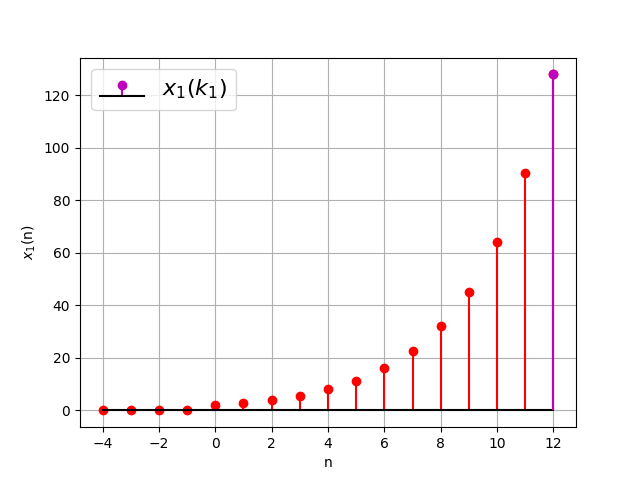
\includegraphics[width=\columnwidth]{ncert-maths/11/9/3/5/figs/a.png}
    \caption[short]{Plot of $x_1$\brak{n} vs n. See \tabref{Table:1}}
    \label{fig:img1}
\end{figure}



\item By \eqref{eq:gsoln}, \eqref{eq:zresult} and \tabref{Table:1}: % prob:b
\begin{align}
    x_2\brak{n} &= x_2\brak{0} r_2^nu\brak{n} \\
    k_2 &= \log_{r_2}{\frac{729}{x_2\brak{0}}} \\
    \therefore k_2 &= 11 \\
    X_2\brak{z} &= \frac{\sqrt{3}}{1 - \sqrt{3}z^{-1}} \quad \abs{z} > \sqrt{3} 
\end{align}

\begin{figure}[h!]
    \renewcommand\thefigure{2}
    \centering
    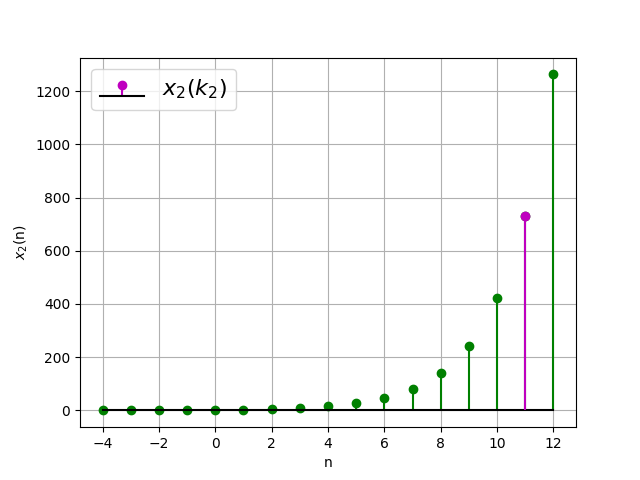
\includegraphics[width=\columnwidth]{ncert-maths/11/9/3/5/figs/b.png}
    \caption[short]{Plot of $x_2$\brak{n} vs n. See \tabref{Table:1}}
    \label{fig:img2}
\end{figure}

\item By \eqref{eq:gsoln}, \eqref{eq:zresult} and \tabref{Table:1}: % prob:c
\begin{align}
    x_3\brak{n} &= x_3\brak{0} r_3^nu\brak{n} \\
    k_3 &= \log_{r_3}{\frac{1}{19683 x_3\brak{0}}} \\
    \therefore k_3 &= 8 \\
    X_3\brak{z} &= \frac{1}{3 - z^{-1}} \quad \abs{z} > \frac{1}{3}
\end{align}

\begin{figure}[h!]
    \renewcommand\thefigure{3}
    \centering
    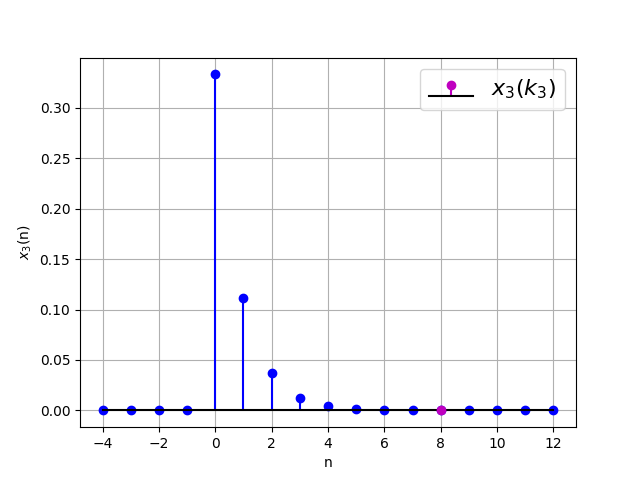
\includegraphics[width=\columnwidth]{ncert-maths/11/9/3/5/figs/c.png}
    \caption[short]{Plot of $x_3$\brak{n} vs n. See \tabref{Table:1}}
    \label{fig:img3}
\end{figure}

\begin{table}[ht]
\begin{tabular}{|c|c|c|}
    \hline 
    \textbf{Parameter}&\textbf{Description} &\textbf{Value}\\
    \hline 
    $r_i$ & Common ratio of G.P (a),(b),(c) & $\sqrt{2}, \sqrt{3}, \frac{1}{3}$ \\
    \hline
    $x_i(0)$ & Initial Values & $2, \sqrt{3}, \frac{1}{3}$ \\
    \hline
    $x_i(k_i)$ & Given Values & $128, 729, \frac{1}{19683}$ \\
    \hline 
    $k_i$ & Desired index & $12, 11, 8$ \\
    \hline 
    $x_i\brak{n}$ & Series & $x_i\brak{0}r_i^nu\brak{n}$ \\
    \hline
	$X_i\brak{z}$ & Z-Transform of $x_i\brak{n}$ & $\frac{x\brak{0}}{1-rz^{-1}}$ \\
    \hline
\end{tabular}

\caption{Table of parameters}
\label{Table:1}


\end{table}

\end{enumerate}

Find the $20^{th}$ and $n^{th}$ terms of the G.P $\frac{5}{2}$, $\frac{5}{4}$, $\frac{5}{8}$,.....

% \item 
% Which term of the following sequences:\\
% (a) 2,$2\sqrt{2}$,4\dots is 128
% \quad(b) $\sqrt{3}$,3,$3\sqrt{3}$\dots is 729\\
% (c) $\frac{1}{3}$,$\frac{1}{9}$,$\frac{1}{27}$\dots is $\frac{1}{19683}$
% \solution
% \iffalse
\let\negmedspace\undefined
\let\negthickspace\undefined
\documentclass[journal,12pt,twocolumn]{IEEEtran}
\usepackage{cite}
\usepackage{amsmath,amssymb,amsfonts,amsthm}
\usepackage{algorithmic}
\usepackage{graphicx}
\usepackage{textcomp}
\usepackage{xcolor}
\usepackage{txfonts}
\usepackage{listings}
\usepackage{enumitem}
\usepackage{mathtools}
\usepackage{gensymb}
\usepackage{comment}
\usepackage[breaklinks=true]{hyperref}
\usepackage{tkz-euclide} 
\usepackage{listings}
\usepackage{gvv}                                        
\def\inputGnumericTable{}                                 
\usepackage[latin1]{inputenc}                                
\usepackage{color}                                            
\usepackage{array}                                            
\usepackage{longtable}                                       
\usepackage{calc}                                             
\usepackage{multirow}                                         
\usepackage{hhline}                                           
\usepackage{ifthen}                                           
\usepackage{lscape}
\usepackage[center]{caption} % center the captions to figure

\newtheorem{theorem}{Theorem}[section]
\newtheorem{problem}{Problem}
\newtheorem{proposition}{Proposition}[section]
\newtheorem{lemma}{Lemma}[section]
\newtheorem{corollary}[theorem]{Corollary}
\newtheorem{example}{Example}[section]
\newtheorem{definition}[problem]{Definition}
\newcommand{\BEQA}{\begin{eqnarray}}
\newcommand{\EEQA}{\end{eqnarray}}
\newcommand{\define}{\stackrel{\triangle}{=}}
\theoremstyle{remark}
\newtheorem{rem}{Remark}
\begin{document}

\newcolumntype{M}[1]{>{\centering\arraybackslash}m{#1}}
\newcolumntype{N}{@{}m{0pt}@{}}

\bibliographystyle{IEEEtran}
\vspace{3cm}

\title{NCERT 11.9.3 5Q} 
\author{ee23btech11223 - Soham Prabhakar More% <-this % stops a space
}
\maketitle
\newpage
\bigskip

\renewcommand{\thefigure}{\theenumi}
\renewcommand{\thetable}{\theenumi}

\bibliographystyle{IEEEtran}

\textbf{Question:}\\
Which term of the following sequences:\\
(a) 2,$2\sqrt{2}$,4\dots is 128
\quad(b) $\sqrt{3}$,3,$3\sqrt{3}$\dots is 729\\
(c) $\frac{1}{3}$,$\frac{1}{9}$,$\frac{1}{27}$\dots is $\frac{1}{19683}$
\fi 
For a general GP series and $k > 0$,
\begin{align}
    x\brak{k} &= x\brak{0}r^k \\
    \therefore k &= \log_r{\frac{x\brak{k}}{x\brak{0}}} \label{eq:gsoln}
\end{align}
And the Z-transform $X\brak{z}$:
\begin{align}
    X\brak{z} &= \frac{x\brak{0}}{1 - rz^{-1}} \quad {\abs{z} > \abs{r}} \label{eq:zresult}
\end{align}

\begin{enumerate}[label=(\alph*)]
\item By \tabref{Table:1}, \eqref{eq:gsoln} and \tabref{Table:1}: % prob:a
\begin{align}
    x_1\brak{n} &= x_1\brak{0} r_1^nu\brak{n} \\
    k_1 &= \log_{r_1}{\frac{128}{x_1\brak{0}}} \\
    \therefore k_1 &= 12 \\
	X_1\brak{z} &= \frac{2}{1 - \sqrt{2}z^{-1}} \quad \abs{z} > \sqrt{2}
\end{align}

\begin{figure}[h!]
    \renewcommand\thefigure{1}
    \centering
    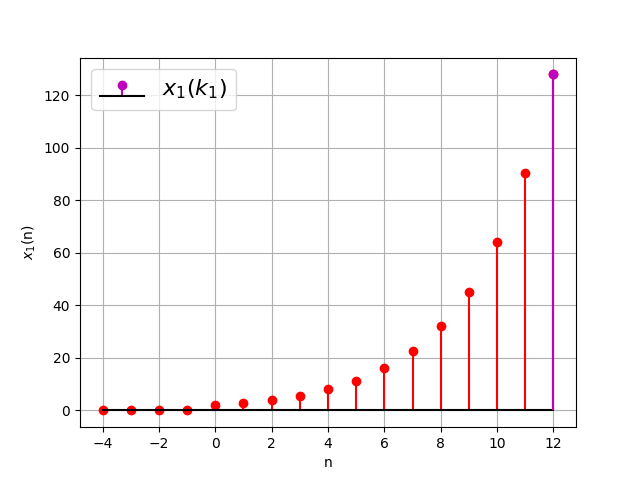
\includegraphics[width=\columnwidth]{ncert-maths/11/9/3/5/figs/a.png}
    \caption[short]{Plot of $x_1$\brak{n} vs n. See \tabref{Table:1}}
    \label{fig:img1}
\end{figure}



\item By \eqref{eq:gsoln}, \eqref{eq:zresult} and \tabref{Table:1}: % prob:b
\begin{align}
    x_2\brak{n} &= x_2\brak{0} r_2^nu\brak{n} \\
    k_2 &= \log_{r_2}{\frac{729}{x_2\brak{0}}} \\
    \therefore k_2 &= 11 \\
    X_2\brak{z} &= \frac{\sqrt{3}}{1 - \sqrt{3}z^{-1}} \quad \abs{z} > \sqrt{3} 
\end{align}

\begin{figure}[h!]
    \renewcommand\thefigure{2}
    \centering
    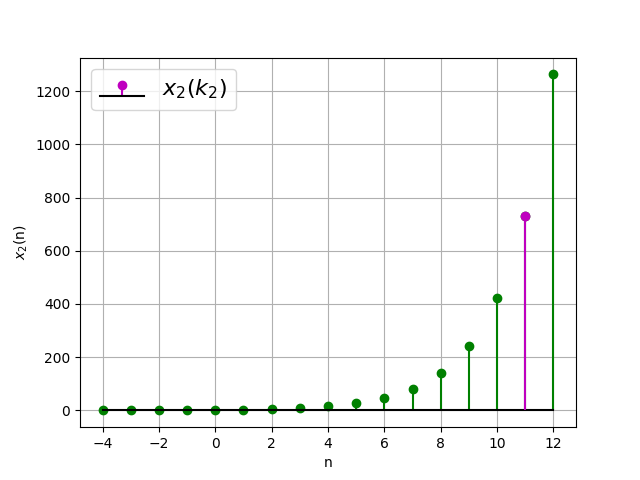
\includegraphics[width=\columnwidth]{ncert-maths/11/9/3/5/figs/b.png}
    \caption[short]{Plot of $x_2$\brak{n} vs n. See \tabref{Table:1}}
    \label{fig:img2}
\end{figure}

\item By \eqref{eq:gsoln}, \eqref{eq:zresult} and \tabref{Table:1}: % prob:c
\begin{align}
    x_3\brak{n} &= x_3\brak{0} r_3^nu\brak{n} \\
    k_3 &= \log_{r_3}{\frac{1}{19683 x_3\brak{0}}} \\
    \therefore k_3 &= 8 \\
    X_3\brak{z} &= \frac{1}{3 - z^{-1}} \quad \abs{z} > \frac{1}{3}
\end{align}

\begin{figure}[h!]
    \renewcommand\thefigure{3}
    \centering
    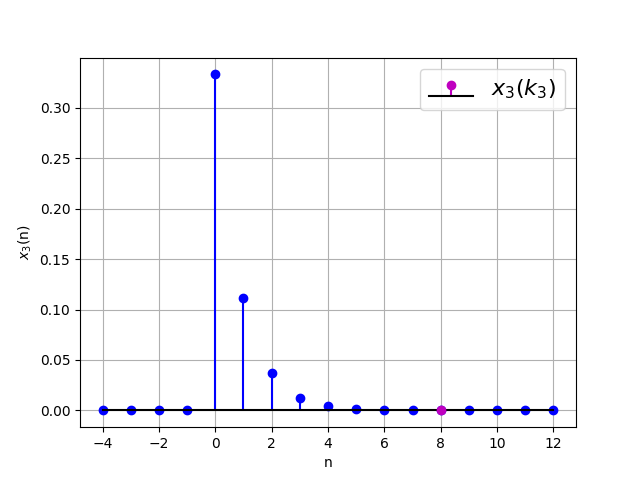
\includegraphics[width=\columnwidth]{ncert-maths/11/9/3/5/figs/c.png}
    \caption[short]{Plot of $x_3$\brak{n} vs n. See \tabref{Table:1}}
    \label{fig:img3}
\end{figure}

\begin{table}[ht]
\input{ncert-maths/11/9/3/5/tables/table.tex}
\end{table}

\end{enumerate}

Find the $20^{th}$ and $n^{th}$ terms of the G.P $\frac{5}{2}$, $\frac{5}{4}$, $\frac{5}{8}$,.....

% \item 
% Which term of the following sequences:\\
% (a) 2,$2\sqrt{2}$,4\dots is 128
% \quad(b) $\sqrt{3}$,3,$3\sqrt{3}$\dots is 729\\
% (c) $\frac{1}{3}$,$\frac{1}{9}$,$\frac{1}{27}$\dots is $\frac{1}{19683}$
% \solution
% \input{ncert-maths/11/9/3/5/main.tex}
% \pagebreak

%\end{document}


% \pagebreak

%\end{document}


% \pagebreak

%\end{document}


\clearpage

\item The number of bacteria in a certain culture doubles every hour. If there were 30 bacteria present in the culture originally, how many bacteria will be present at the end of $2^{nd}$ hour, $4^{th}$ hour and $n^{th}$ hour?

\solution
\iffalse
\let\negmedspace\undefined
\let\negthickspace\undefined
\documentclass[journal,12pt,twocolumn]{IEEEtran}
\usepackage{cite}
\usepackage{amsmath,amssymb,amsfonts,amsthm}
\usepackage{algorithmic}
\usepackage{graphicx}
\usepackage{textcomp}
\usepackage{xcolor}
\usepackage{txfonts}
\usepackage{listings}
\usepackage{enumitem}
\usepackage{mathtools}
\usepackage{gensymb}
\usepackage{comment}
\usepackage[breaklinks=true]{hyperref}
\usepackage{tkz-euclide}
\usepackage{listings}
\usepackage{gvv}
\def\inputGnumericTable{}
\usepackage[latin1]{inputenc}
\usepackage{color}
\usepackage{array}
\usepackage{longtable}
\usepackage{calc}
\usepackage{multirow}
\usepackage{hhline}
\usepackage{ifthen}
\usepackage{lscape}

\newtheorem{theorem}{Theorem}[section]
\newtheorem{problem}{Problem}
\newtheorem{proposition}{Proposition}[section]
\newtheorem{lemma}{Lemma}[section]
\newtheorem{corollary}[theorem]{Corollary}
\newtheorem{example}{Example}[section]
\newtheorem{definition}[problem]{Definition}
\newcommand{\BEQA}{\begin{eqnarray}}
\newcommand{\EEQA}{\end{eqnarray}}
\newcommand{\define}{\stackrel{\triangle}{=}}
\theoremstyle{remark}
\newtheorem{rem}{Remark}
\begin{document}

\bibliographystyle{IEEEtran}
\vspace{3cm}

\title{NCERT Discrete - 11.9.3.30}
\author{EE23BTECH11007 - Aneesh Kadiyala$^{*}$% <-this % stops a space
}
\maketitle
\newpage
\bigskip

\renewcommand{\thefigure}{\theenumi}
\renewcommand{\thetable}{\theenumi}

\vspace{3cm}
\textbf{Question 11.9.3.30:} The number of bacteria in a certain culture doubles every hour. If there were 30 bacteria present in the culture originally, how many bacteria will be present at the end of $2^{nd}$ hour, $4^{th}$ hour and $n^{th}$ hour?
\\
\solution
\fi
\begin{table}[h!]
    \begin{tabular}{ | c | c | c | }
    \hline
    Parameter & Value & Description \\
    \hline
    $x(0)$ & 30 & Initial no. of bacteria\\
    \hline
    $r$ & 2 & Ratio of no. of bacteria at end of \\
    & & hour to start of hour (Common Ratio) \\
    \hline
    $x(n)$ & $r^nx(0)u(n)$ & $n^{th}$ term of the GP \\
    \hline
\end{tabular}
    \caption{Input Parameters}
    \label{tab:ncert_maths_11_9_3_30}
\end{table}
From \tabref{tab:ncert_maths_11_9_3_30}:
\begin{align}
x(2) &= 120 \\
x(4) &= 480 \\
x(n) &= 30(2^n)u(n)
\end{align}
\begin{figure}[h!]
    \centering
    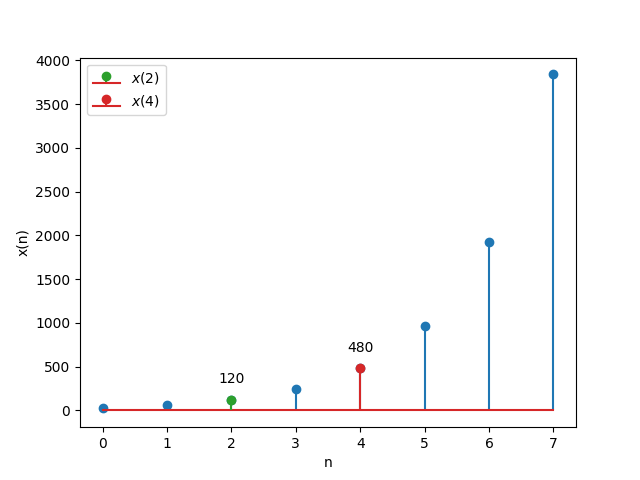
\includegraphics[width=\columnwidth]{ncert-maths/11/9/3/30/figs/11_9_3_30.png}
    \caption{Plot of $x(n)$ vs $n$. See \tabref{tab:ncert_maths_11_9_3_30} for details.}
    \label{fig:ncert_maths_11_9_3_30}
\end{figure}
\begin{align}
X(z) = \frac{30z^{-1}}{1 - 2z^{-1}} \quad \abs{z} > 2
\end{align}
%\end{document}


\item Ramkali saved Rs 5 in the first week of a year and then increased her weekly savings by Rs 1.75. If in the $n$th week, her weekly savings become Rs 20.75, find $n$.

\solution
\iffalse
\let\negmedspace\undefined
\let\negthickspace\undefined
\documentclass[journal,12pt,twocolumn]{IEEEtran}
\usepackage{cite}
\usepackage{amsmath,amssymb,amsfonts,amsthm}
\usepackage{algorithmic}
\usepackage{graphicx}
\usepackage{textcomp}
\usepackage{xcolor}
\usepackage{txfonts}
\usepackage{listings}
\usepackage{enumitem}
\usepackage{mathtools}
\usepackage{gensymb}
\usepackage[breaklinks=true]{hyperref}
\usepackage{tkz-euclide} % loads  TikZ and tkz-base
\usepackage{listings}
\usepackage{gvv}


\newtheorem{theorem}{Theorem}[section]
\newtheorem{problem}{Problem}
\newtheorem{proposition}{Proposition}[section]
\newtheorem{lemma}{Lemma}[section]
\newtheorem{corollary}[theorem]{Corollary}
\newtheorem{example}{Example}[section]
\newtheorem{definition}[problem]{Definition}

\newcommand{\BEQA}{\begin{eqnarray}}
\newcommand{\EEQA}{\end{eqnarray}}
\newcommand{\define}{\stackrel{\triangle}{=}}
\theoremstyle{remark}
\newtheorem{rem}{Remark}

\graphicspath{./figs/}

%\bibliographystyle{ieeetr}
\begin{document}
%

\bibliographystyle{IEEEtran}


\vspace{3cm}

\title{
	%	\logo{
	Assignment-1 

	\large{EE:1205 Signals and Systems}

	Indian Institute of Technology, Hyderabad
	%	}
}
\author{Kunal Thorawade

EE23BTECH11035
}	

\maketitle


\newpage

%\tableofcontents

\bigskip
 
 \renewcommand{\thefigure}{\theenumi}
 \renewcommand{\thetable}{\theenumi}
 %\renewcommand{\theequation}{\theenumi}

 \section{\Large Question:}  Ramkali saved Rs 5 in the first week of a year and then increased her weekly savings by Rs 1.75. If in the $n$th week, her weekly savings become Rs 20.75, find $n$.

 \section{\Large Solution:} 
 \fi
 \begin{table}[ht]
    \centering
    \begin{tabular}{|c|c|c|}
        \hline
        Parameter & Value & Description \\
        \hline
        $x(0)$ & 5 & First term of AP \\
        $d$ & 1.75 & Common difference of AP \\
        $x(n)$ & 20.75 & $n^{th}$ term of AP \\
        \hline
    \end{tabular}
    \vspace{2mm}
    \caption{Parameter List}
    \label{tab:simple.10.5.2.20}
\end{table}


 \begin{align} 
	 x(n) &= x(0) + (n)(d)
	 \\ 20.75 &= 5 + (n)(1.75)  
	 \\ \implies 15.75 &= (n)(1.75)
	 \\ \implies n &= \frac{15.75}{1.75}
	 \\ \implies n &= 9
	 \\x(n) &= 5u(n) + 1.75nu(n)
 \end{align}
 The Z-transform of a sequence $x(n)$ is given by:
 \begin{align}
	  X(z) &= \frac{5z^{-1}}{1-z^{-1}}+\frac{1.75z^{-1}}{(1-z^{-1})^{2}} ; |z| > 1
 \end{align}

 \begin{figure}
	     \centering
	         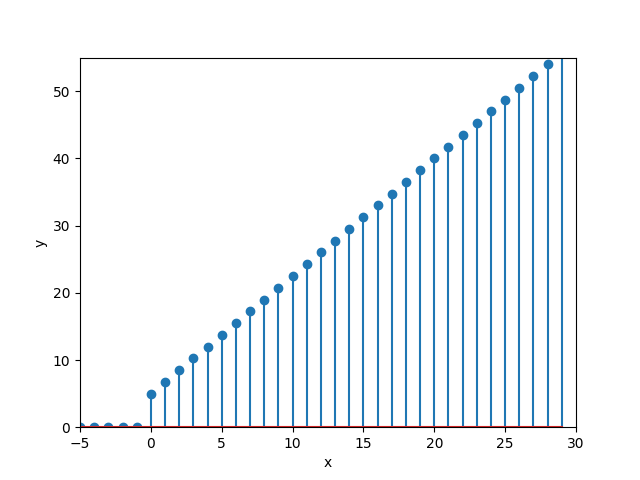
\includegraphics[width = 8cm]{ncert-maths/10/5/2/20/figs/fig1.png}
		     \caption{Plot of $x(n) = 5 + 1.75n$}
		         \label{fig:enter-label.10.5.2.20}
 \end{figure}




\item Show that the sum of $\brak {m+n}^{th}$ and $\brak {m-n}^{th}$ terms of an $A.P.,$ is equal to twice the $m^{th}$ terms.    \\
\solution
\iffalse
\let\negmedspace\undefined
\let\negthickspace\undefined
\documentclass[journal,12pt,twocolumn]{IEEEtran}
\usepackage{cite}
\usepackage{amsmath,amssymb,amsfonts,amsthm}
\usepackage{algorithmic}
\usepackage{graphicx}
\usepackage{textcomp}
\usepackage{xcolor}
\usepackage{txfonts}
\usepackage{listings}
\usepackage{enumitem}
\usepackage{mathtools}
\usepackage{gensymb}
\usepackage{comment}
\usepackage[breaklinks=true]{hyperref}
\usepackage{tkz-euclide} 
\usepackage{listings}
\usepackage{gvv}                                        
\def\inputGnumericTable{}                                 
\usepackage[latin1]{inputenc}                                
\usepackage{color}                                            
\usepackage{array}                                            
\usepackage{longtable}                                       
\usepackage{calc}                                             
\usepackage{multirow}                                         
\usepackage{hhline}                                           
\usepackage{ifthen}                                           
\usepackage{lscape}

\newtheorem{theorem}{Theorem}[section]
\newtheorem{problem}{Problem}
\newtheorem{proposition}{Proposition}[section]
\newtheorem{lemma}{Lemma}[section]
\newtheorem{corollary}[theorem]{Corollary}
\newtheorem{example}{Example}[section]
\newtheorem{definition}[problem]{Definition}
\newcommand{\BEQA}{\begin{eqnarray}}
\newcommand{\EEQA}{\end{eqnarray}}
\newcommand{\define}{\stackrel{\triangle}{=}}
\theoremstyle{remark}
\newtheorem{rem}{Remark}
\begin{document}
\parindent 0px
\bibliographystyle{IEEEtran}
\title{Assignment 11.9.5\_1Q}
\author{EE22BTECH11219 - Rada Sai Sujan$^{}$% <-this % stops a space
}
\maketitle
\newpage
\bigskip
\section*{Question}
Show that the sum of $\brak {m+n}^{th}$ and $\brak {m-n}^{th}$ terms of an $A.P.,$ is equal to twice the $m^{th}$ terms.    \\
\solution
\fi

\begin{table}[ht]
    \centering
    \def\arraystretch{1.5}
    \begin{tabular}{|p{2cm}|p{2.5cm}|p{2.3cm}|}
    \hline
    PARAMETER & VALUE & DESCRIPTION  \\ \hline
    $$x\brak0$$ & $$x\brak{0}$$ & First term \\ \hline
    $$d$$ & $$d$$ & common difference \\ \hline
    $$x(n)$$ & $$[x\brak{0}+nd]u\brak n$$ & General term of the series  \\ \hline
  \end{tabular}

    \caption{Parameter Table1}
    \label{tab:10.9.5.1.1}
\end{table}
For an $AP$,
\begin{align}
    x\brak{n}&=[x\brak{0}+nd]u\brak{n}   \\
    \implies x\brak{m+n}+x\brak{m-n}&=[x\brak{0}+\brak{m+n}d]+[x\brak{0}+\brak{m-n}d] \\
    &=2[x\brak{0}+md]   \\
    \therefore x\brak{m+n}+x\brak{m-n}&=2x\brak{m}
\end{align}
\begin{table}[ht]
    \centering
    \def\arraystretch{1.5}
    \begin{tabular}{|p{4.5cm}|p{4.5cm}|}
    \hline
      $$x\brak{0}$$ & $$3$$  \\ \hline
      $$d$$ & $$2$$  \\ \hline
      $$m$$ & $$6$$  \\ \hline
      $$n$$ & $$2$$  \\ \hline
      $$x\brak{m+n}$$ & $$19$$  \\ \hline
      $$x\brak{m-n}$$ & $$11$$  \\ \hline
      $$x\brak{m}$$ & $$15$$  \\ \hline
    \end{tabular}

    \caption{Verified Values}
    \label{tab:10.9.5.1.2}
\end{table}




\item The sum of the first three terms of a G.P is $39/10$ and their product is $1$. Find the common ratio and the terms.\\
\solution
\iffalse
\let\negmedspace\undefined
\let\negthickspace\undefined
\documentclass[journal,12pt,twocolumn]{IEEEtran}
\usepackage{cite}
\usepackage{amsmath,amssymb,amsfonts,amsthm}
\usepackage{algorithmic}
\usepackage{graphicx}
\usepackage{textcomp}
\usepackage{xcolor}
\usepackage{txfonts}
\usepackage{listings}
\usepackage{enumitem}
\usepackage{mathtools}
\usepackage{gensymb}
\usepackage{comment}
\usepackage[breaklinks=true]{hyperref}
\usepackage{tkz-euclide}
\usepackage{listings}
\usepackage{gvv}
\def\inputGnumericTable{}
\usepackage[latin1]{inputenc}
\usepackage{color}
\usepackage{array}
\usepackage{longtable}
\usepackage{calc}
\usepackage{multirow}
\usepackage{hhline}
\usepackage{ifthen}
\usepackage{lscape}

\newtheorem{theorem}{Theorem}[section]
\newtheorem{problem}{Problem}
\newtheorem{proposition}{Proposition}[section]
\newtheorem{lemma}{Lemma}[section]
\newtheorem{corollary}[theorem]{Corollary}
\newtheorem{example}{Example}[section]
\newtheorem{definition}[problem]{Definition}
\newcommand{\BEQA}{\begin{eqnarray}}
\newcommand{\EEQA}{\end{eqnarray}}
\newcommand{\define}{\stackrel{\triangle}{=}}
\theoremstyle{remark}
\newtheorem{rem}{Remark}
\begin{document}

\bibliographystyle{IEEEtran}
\vspace{3cm}

\title{NCERT Discrete - 11.9.3.12}
\author{EE23BTECH11058 - Sindam Ananya$^{*}$% <-this % stops a space
}
\maketitle
\newpage
\bigskip

\renewcommand{\thefigure}{\theenumi}
\renewcommand{\thetable}{\theenumi}

\vspace{3cm}
\textbf{Question : 11.9.3.12} 
The sum of the first three terms of a G.P is $39/10$ and their product is $1$. Find the common ratio and the terms.\\
\solution
\fi
\begin{table}[h!]
    \centering
    \begin{tabular}{|c|c|c|}
        \hline
        \textbf{Parameter} & \textbf{Value} & \textbf{Description} \\
        \hline
        $x(0)$ & & First term \\
        \hline
        $r$ & & Common ratio \\
        \hline
        $x(0)^3r^3$ & 1 & Product of terms \\
        \hline
        $x(0)$ + $x(0)r$ + $x(0)r^2$ & $\frac{39}{10}$ & Sum of terms \\
        \hline
    \end{tabular}

    \caption{Input Parameters}
    \label{tab:11.9.3.12table1}
\end{table}
\begin{equation}
y(n) = x(0)\brak{\frac{r^{n+1}-1}{r-1}}u(n)
\label{eq:11.9.3.12eq1}
\end{equation}
From \tabref{tab:11.9.3.12table1} and \eqref{eq:11.9.3.12eq1} :
\begin{align}
y(2) &= x(0)\brak{\frac{r^3-1}{r-1}}\\
\frac{39}{10} &= x(0)\brak{r^2+r+1}\\
\implies \frac{39r}{10} &= r^2+r+1 \quad \brak{\because x(0)r = 1}\\
\implies (2r-5)(5r-2) &=0\\
\implies r &= \frac{2}{5} \quad or \quad \frac{5}{2}
\end{align}
\begin{enumerate}
      \item If $r = \frac{2}{5}$, then terms are $\frac{5}{2}$, $1$, $\frac{2}{5}$.
      \item If $r = \frac{5}{2}$, then terms are $\frac{2}{5}$, $1$, $\frac{5}{2}$.
\end{enumerate}
\begin{figure}[h!]
    \centering
    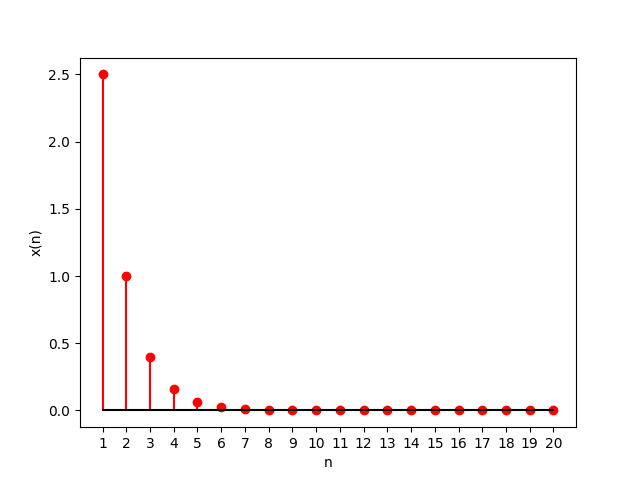
\includegraphics[width=\columnwidth]{ncert-maths/11/9/3/12/figs/graph1.png}
    \caption{stem plots of GP if $r=\frac{2}{5}$}
    \label{fig:11.9.3.12_1}
\end{figure}
\begin{figure}[h!]
    \centering
    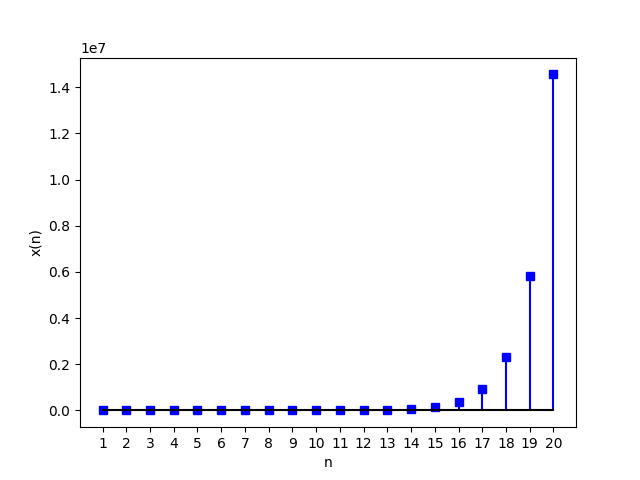
\includegraphics[width=\columnwidth]{ncert-maths/11/9/3/12/figs/graph2.png}
    \caption{stem plots of GP if $r=\frac{5}{2}$}
    \label{fig:11.9.3.12_2}
\end{figure}
%\end{document}




\item The ratio of the A.M and G.M of two positive numbers $a$ and $b$ is $m:n$. Show that $a:b = \brak{ m + \sqrt{m^2 - n^2}} : \brak{ m - \sqrt{m^2 - n^2}}$.\\
\solution
\let\negmedspace\undefined
\let\negthickspace\undefined
\documentclass[journal,12pt,onecolumn]{IEEEtran}
\usepackage{cite}
\usepackage{amsmath,amssymb,amsfonts,amsthm}
\usepackage{algorithmic}
\usepackage{graphicx}
\usepackage{textcomp}
\usepackage{xcolor}
\usepackage{txfonts}
\usepackage{listings}
\usepackage{enumitem}
\usepackage{mathtools}
\usepackage{gensymb}

\usepackage{tkz-euclide} % loads  TikZ and tkz-base
\usepackage{listings}



\newtheorem{theorem}{Theorem}[section]
\newtheorem{problem}{Problem}
\newtheorem{proposition}{Proposition}[section]
\newtheorem{lemma}{Lemma}[section]
\newtheorem{corollary}[theorem]{Corollary}
\newtheorem{example}{Example}[section]
\newtheorem{definition}[problem]{Definition}
%\newtheorem{thm}{Theorem}[section] 
%\newtheorem{defn}[thm]{Definition}
%\newtheorem{algorithm}{Algorithm}[section]
%\newtheorem{cor}{Corollary}
\newcommand{\BEQA}{\begin{eqnarray}}
\newcommand{\EEQA}{\end{eqnarray}}
\newcommand{\system}[1]{\stackrel{#1}{\rightarrow}}

\newcommand{\define}{\stackrel{\triangle}{=}}
\theoremstyle{remark}
\newtheorem{rem}{Remark}
%\bibliographystyle{ieeetr}
\begin{document}
%
\providecommand{\pr}[1]{\ensuremath{\Pr\left(#1\right)}}
\providecommand{\prt}[2]{\ensuremath{p_{#1}^{\left(#2\right)} }}        % own macro for this question
\providecommand{\qfunc}[1]{\ensuremath{Q\left(#1\right)}}
\providecommand{\sbrak}[1]{\ensuremath{{}\left[#1\right]}}
\providecommand{\lsbrak}[1]{\ensuremath{{}\left[#1\right.}}
\providecommand{\rsbrak}[1]{\ensuremath{{}\left.#1\right]}}
\providecommand{\brak}[1]{\ensuremath{\left(#1\right)}}
\providecommand{\lbrak}[1]{\ensuremath{\left(#1\right.}}
\providecommand{\rbrak}[1]{\ensuremath{\left.#1\right)}}
\providecommand{\cbrak}[1]{\ensuremath{\left\{#1\right\}}}
\providecommand{\lcbrak}[1]{\ensuremath{\left\{#1\right.}}
\providecommand{\rcbrak}[1]{\ensuremath{\left.#1\right\}}}
\newcommand{\sgn}{\mathop{\mathrm{sgn}}}
\providecommand{\abs}[1]{\left\vert#1\right\vert}
\providecommand{\res}[1]{\Res\displaylimits_{#1}} 
\providecommand{\norm}[1]{\left\lVert#1\right\rVert}
%\providecommand{\norm}[1]{\lVert#1\rVert}
\providecommand{\mtx}[1]{\mathbf{#1}}
\providecommand{\mean}[1]{E\left[ #1 \right]}
\providecommand{\cond}[2]{#1\middle|#2}
\providecommand{\fourier}{\overset{\mathcal{F}}{ \rightleftharpoons}}
\newenvironment{amatrix}[1]{%
  \left(\begin{array}{@{}*{#1}{c}|c@{}}
}{%
  \end{array}\right)
}
%\providecommand{\hilbert}{\overset{\mathcal{H}}{ \rightleftharpoons}}
%\providecommand{\system}{\overset{\mathcal{H}}{ \longleftrightarrow}}
	%\newcommand{\solution}[2]{\textbf{Solution:}{#1}}
\newcommand{\solution}{\noindent \textbf{Solution: }}
\newcommand{\cosec}{\,\text{cosec}\,}
\providecommand{\dec}[2]{\ensuremath{\overset{#1}{\underset{#2}{\gtrless}}}}
\newcommand{\myvec}[1]{\ensuremath{\begin{pmatrix}#1\end{pmatrix}}}
\newcommand{\mydet}[1]{\ensuremath{\begin{vmatrix}#1\end{vmatrix}}}
\newcommand{\myaugvec}[2]{\ensuremath{\begin{amatrix}{#1}#2\end{amatrix}}}
\providecommand{\rank}{\text{rank}}
\providecommand{\pr}[1]{\ensuremath{\Pr\left(#1\right)}}
\providecommand{\qfunc}[1]{\ensuremath{Q\left(#1\right)}}
	\newcommand*{\permcomb}[4][0mu]{{{}^{#3}\mkern#1#2_{#4}}}
\newcommand*{\perm}[1][-3mu]{\permcomb[#1]{P}}
\newcommand*{\comb}[1][-1mu]{\permcomb[#1]{C}}
\providecommand{\qfunc}[1]{\ensuremath{Q\left(#1\right)}}
\providecommand{\gauss}[2]{\mathcal{N}\ensuremath{\left(#1,#2\right)}}
\providecommand{\diff}[2]{\ensuremath{\frac{d{#1}}{d{#2}}}}
\providecommand{\myceil}[1]{\left \lceil #1 \right \rceil }
\newcommand\figref{Fig.~\ref}
\newcommand\tabref{Table~\ref}
\newcommand{\sinc}{\,\text{sinc}\,}
\newcommand{\rect}{\,\text{rect}\,}
%%
%	%\newcommand{\solution}[2]{\textbf{Solution:}{#1}}
%\newcommand{\solution}{\noindent \textbf{Solution: }}
%\newcommand{\cosec}{\,\text{cosec}\,}
%\numberwithin{equation}{section}
%\numberwithin{equation}{subsection}
%\numberwithin{problem}{section}
%\numberwithin{definition}{section}
%\makeatletter
%\@addtoreset{figure}{problem}
%\makeatother

%\let\StandardTheFigure\thefigure
\let\vec\mathbf

\bibliographystyle{IEEEtran}





\bigskip

\renewcommand{\thefigure}{\theenumi}
\renewcommand{\thetable}{\theenumi}
%\renewcommand{\theequation}{\theenumi}


\title{Discrete Assignment}
\author{Karyampudi Meghana Sai\\ EE23BTECH11031}
\maketitle



The ratio of the A.M and G.M of two positive numbers $a$ and $b$ is $m:n$. Show that $a:b = \brak{ m + \sqrt{m^2 - n^2}} : \brak{ m - \sqrt{m^2 - n^2}}$.\\
\solution

Expressing A.M and G.M in terms of $a$ and $b$:
\begin{align}
\frac{a + b}{2\sqrt{ab}} = \frac{m}{n} \label{eq:11.9.5.19eq1}
\end{align}

Let's assume that $x = \sqrt{\frac{a}{b}}$. Then, we have:
\begin{align}
\frac{a}{b} = x^2 \label{eq:11.9.5.19eq2}
\end{align}

Substituting the value of x in equation \eqref{eq:11.9.5.19eq1}:
\begin{align}
\frac{1 + x^2}{2x} &= \frac{m}{n}\label{eq:11.9.5.19eq3} \\
\frac{1}{x} + x &= \frac{2m}{n} \label{eq:11.9.5.19eq4} \\
x^2 - \frac{2m}{n}x + 1 &=  0 \label{eq:11.9.5.19eq5}\\
\implies x &= \frac{m}{n} \pm \frac{\sqrt{m^2 - n^2}}{n} \label{eq:11.9.5.19eq6}
\end{align}

Since $x = \sqrt{\frac{a}{b}}$, $x$ must be positive.
\begin{align}
x = \frac{m + \sqrt{m^2 - n^2}}{n}\label{eq:11.9.5.19eq7}
\end{align}

Referencing the value of $x$ from equation\eqref{eq:11.9.5.19eq2}.
\begin{align}
\frac{a}{b} &=\brak{\frac{m + \sqrt{m^2 - n^2}}{n}}^2  \label{eq:11.9.5.19eq8}
\end{align}

Multiplying both the numerator and denominator with $\brak{m-\sqrt{m^2 - n^2}}$: 
\begin{align} 
\frac{a}{b} &= \frac{1}{n^2} \frac{\brak{m + \sqrt{m^2 - n^2}}^2  \brak{m-\sqrt{m^2 - n^2}}}{\brak{m-\sqrt{m^2 - n^2}}}\label{eq:11.9.5.19eq9}\\
\implies a:b &= \brak{ m + \sqrt{m^2 - n^2}}: \brak{m - \sqrt{m^2 - n^2}}\label{eq:11.9.5.19eq10}
\end{align}
nth term of the AP :
\begin{align}
y(n)&=\sbrak{a+n\brak{b-a}}u(n)\label{eq:11.9.5.19eq11}\\
n^k u(n) &\system{Z} (-1)^k z^k \frac{d^k}{dz^k}U(z)\label{eq:11.9.5.19eq12}\\
u(n) &\system{Z} \frac{1}{\brak{1 - z^{-1}}} \quad \abs{ z} > \abs{1} \label{eq:11.9.5.19eq13}\\
nu(n) &\system{Z} \frac{z^{-1}}{\brak{1 - z^{-1}}^2} \quad \abs{ z} > \abs{1} \label{eq:11.9.5.19eq14}
\end{align}
Referencing the equations from \eqref{eq:11.9.5.19eq13},\eqref{eq:11.9.5.19eq14}.\\
\begin{align}
y(n) &\system{Z} \frac{a}{\brak{1 - z^{-1}}}+\frac{\brak{b-a}z^{-1}}{\brak{1-z^{-1}}^2} \quad \abs{ z} > \abs{1} \label{eq:11.9.5.19eq15}
\end{align}
nth term of the GP :
\begin{align}
y(n)&=a\brak{{\frac{b}{a}}}^n u(n)\label{eq:11.9.5.19eq16}\\
r^n u(n) &\system{Z} \frac{1}{\brak{1-rz^{-1}}} \quad \abs{ z} > \abs{r} \label{eq:11.9.5.19eq17}
\end{align}
Referencing the equation from \eqref{eq:11.9.5.19eq17}.\\
\begin{align}
y(n) &\system{Z} \frac{a^2 z^{-1}}{\brak{a-bz^{-1}}} \quad \abs{ z} > \abs{\frac{b}{a}}\label{eq:11.9.5.19eq18}
\end{align}
\end{document}



\item The sum of three numbers in an arithmetic progression (AP) is $24$ and the product of those three numbers is $440$, find the values of the three numbers.\\
\solution

\item The sum of some terms of G.P. is $315$ whose first term and the common ratio are $5$ and $2$ , respectively. Find the last term and the number of terms.\\
\solution

\end{enumerate}
